\documentclass[twocolumn,prl,nobalancelastpage,aps,10pt,floatfix]{revtex4-1}

%\documentclass[rmp,preprint]{revtex4-1} 
\usepackage{graphicx,bm,times, float} 

\usepackage[caption = false]{subfig}
\usepackage[demo]{graphicx}

\begin{document} 
 
\title{A Study of Van Allen Belt Signatures of Nuclear Weapon Tests for Future CTBT
Technologies} 
 
\author{Filip M. Wach} 
 
\affiliation{Department of Physics, University of Bristol.} 
 
\begin{abstract} One of the methods of enforcing the Comprehensive Test Ban Treaty (CTBT) involves complementary measurements of seismic signals. Data from low Earth orbit satellites show that seismic events can result in particle bursts which can be detected by sensors on board of satellites.  There is strong evidence for precipitation of charged particles in the van Allen belts caused by seismic events. Coincident particle bursts in satellite-borne detectors have been observed with a $>$ 5-sigma significance with earthquake activity at the corresponding location in SAMPEX/PET, MARIA/SALYUT--7, GAMMA--1 \cite{alex}, and DEMETER \cite{dem}. The mechanism responsible for particle precipitation can be linked to acoustic gravity wave causing Ultra Low Frequency (ULF) charge oscillation in ionosphere coupling to the magnetosphere through travelling Alfven waves around the Earth's dipolar field \cite{siv}. This same mechanism is also expected for underground nuclear tests. The main objective of this project is to study the signatures of nuclear weapon tests performed by North Korea in 2006, 2009, 2013 and 2016, and ultimately to discern natural earthquake phenomena from nuclear tests.
	 
 
\end{abstract} 
\date{\today} 
 
\maketitle 
 
\section{INTRODUCTION} 
 
The mechanism leading to particle bursts (PBs) is believed to be caused by the Ultra and Extra Low Frequency (ULF and ELF) waves emissions. These waves are believed to be caused by a range of preseismic sources such as local deformation of field electro-kinetics, piezo-magnetism and piezoelectricity and many others \cite{siv}. 
Both \textit{Sivadas} and \textit{Aleksandrin} propose that these low frequency waves become trapped in a geomagnetic field tube (specific channel made by L--shell corresponding to the earthquake) on altitudes between 300 -- 500 km. They then travel as magneto--hydrodynamic Alfven waves along the given L--shell interacting resonantly with particles trapped within that region (depending on frequency of the emission these are bounce resonance or cyclotron resonance interactions). This ultimately results in particles precipitating and circulating within their given L--shell for up to 12 hours.

The data for this project comes from Los Almost National Laboratory and was collected by 23 GPS satellites between 1\textsuperscript{st} January 2001 and 1\textsuperscript{st} January 2017. The satellites were equipped with with Burst Detector Dosimeters IIR (BDD-IIR) \cite{tusz1} and Combined X-Ray sensor and Dosimeters (CXD) \cite{tusz2} and travelled along a path with a period of approximately 12 hours, taking measurements every 240s. Figure \ref{tr} shows trajectories of some of the GPS satellites.
\begin{figure} 
	\includegraphics*[width=0.96\linewidth,clip]{trajectories} 
	\caption{Trajectories of satellites equipped with CXD instruments \cite{mor}.}\label{tr} 
\end{figure}

 Particle detectors took measurements of rates and fluxes for both electrons and protons as well as recorded geographic locations, magnetic fields and L--shell values. In this analysis we foucsed mainly on electron rates and their variation in time and within L--shells.
 
\section{Method} 


\subsection{Correlated particle bursts and surrogate seismic events}

In this part of the project we investigated whether the observations made by low--Earth--orbit satellites can also be found in our data. In our analysis we attempted to reproduce the results presented by \textit{Aleksandrin et al.} by imporoving his analysis method.

The data was analysed in two--year chunks and PBs were defined as readings exceeding the average by at least four $\sigma$. Subsequently, PBs were matched to earthquakes (obtained from U.S. Geological Survey website) based on the following conditions: PB occurs within 12 hours before or after the earthquake and the relationship between the earthquake L--Shell (L\textsubscript{EQ}) and burst L--shell (L\textsubscript{PB}) 
can be described by
\begin{equation}  
\Delta L = L\textsubscript{EQ} - L\textsubscript{PB} < 0.07 
\end{equation}
Since precipitated particles remain trapped witin a given L--Shell for up to 12 hours, we assume that detection of PB depends only on the L--Shells the satellite is traversing regardless of its geographic locatin.

\subsection{Energy spectrum cross--correlation analyis} 

This method involved investigating normalised cross--correlation coefficients (NCC) between various electron energy channels.
\begin{equation}
NCC = \frac{\sum_{n=0}^{N}x(n)\sum_{n=0}^{N}y(n)}{\sqrt{\sum_{n=0}^{N}x^2(n)\sum_{n=0}^{N}y^2(n)}}
\end{equation}
Figure \ref{bkg} shows a typical weekly set of readings.
\begin{figure}
\includegraphics*[width=0.96\linewidth,clip]{bkg2} 
\caption{Figure to show L--Shell, proton and electron rate readings between 24\textsuperscript{th} Sept and 31\textsuperscript{st} Sept 2010.}\label{bkg} 
\end{figure}
By investigating NCCs for 2--week periods over 16 years of data, overall 'distribution' can be obtained in order to use this population as the baseline for comparison with periods of nuclear activity.
 
\section{RESULTS} 
Figure \ref{test} shows data collected around one of the nuclear tests.
\begin{figure} 
	\includegraphics*[width=0.96\linewidth,clip]{test} 
	\caption{Electron and proton rates for the test on 25\textsuperscript{th} May 2006 (marked by black vertical line).}\label{test} 
\end{figure} 
An example of temporal histogram is shown in Figure \ref{temp}. The peaks are representing particle bursts detected by the satellite. The coupling between the earthquake and PB usually occurs around 4 $<$ L--shell $<$ 5.
\begin{figure} 
	\includegraphics*[width=0.96\linewidth,clip]{Temp_correlation_ns56(2)} 
	\caption{Temporal correlation histogram for satellite ns56 under the condition $\Delta$L $<$ 0.07.}\label{temp} 
\end{figure} 
By increasing the allowed values of $\Delta$L the features become much less distinguishible as seen in Figure \ref{temp_largeL}. These patterns show findings described in literature.
\begin{figure} 
	\includegraphics*[width=0.96\linewidth,clip]{temp_largeL} 
	\caption{Temporal correlation histogram for satellite ns56 under the condition $\Delta$L $<$ 1  .}\label{temp_largeL} 
\end{figure}

Method of energy spectrum cross--correlation analysis appeared to be succesfull in discerning between nuclear tests from 2006, 2009 and 2013 and naturally occuring phenomena. Figure \ref{Xcor} shows a histogram of how a set of NCCs for a particular test from 25\textsuperscript{th} May 2006 compare to the overall population and table \ref{pv} gives the set of p--values for all the channels for this test.
\begin{figure}
	\includegraphics*[width=0.96\linewidth,clip]{Xcor_54(2)} 
	\caption{NCC between channels 2 and 4 for a test performed on 25\textsuperscript{th} May 2006 as compared to the values calculated for 16 years of data.}\label{Xcor} 
\end{figure}
 \begin{table}
 	\begin{tabular}{|c|c|c|c|c|c|c|c|c|c|c|c|}
 		\hline
 		Channel & 0 & 1 & 2 & 3 & 4 & 5 & 6 & 7 & 8 & 9 & 10  \\
 		\hline
 		P--values & 0.49 & 0.72 & 1.00 & 0.01 & 0.01 & 0.04 & 0.04 & 0.07 & 0.05 & 0.03 & 0.03\\
 		\hline	
 	\end{tabular}
 \caption{Table of P--values for NCCs from the test performed on 25\textsuperscript{th} May 2006.}\label{pv} 
 \end{table}

This method was applied to data collected by five different satellites. An outlying p--value is defined as lower than 0.05. Table \ref{Xsat} shows the number of outliers for each nuclear test recorder by the satellites.

\begin{table}[]
	\centering
	\caption{Number of observed outliers by satellites for different nuclear tests.}\label{Xsat}
	\begin{tabular}{l|l|l|l|l|l|}
		\cline{2-6}
		& ns54 & ns56 & ns59 & ns60 & ns61  \\ \hline
		\multicolumn{1}{|l|}{Oct 2006} & 1 & 0 & 0 & 1 & 1 \\ \hline
		\multicolumn{1}{|l|}{May 2009} & 6 & 2 & 1 & 2 & 2 \\ \hline
		\multicolumn{1}{|l|}{Feb 2013} & 3 & 4 & 4 & 2 & 3 \\ \hline
		\multicolumn{1}{|l|}{Jan 2016} & 0 & 0 & 0 & 0 & 0 \\ \hline
		\multicolumn{1}{|l|}{Sep 2016} & 0 & 0 & 0 & 0 & 0 \\ \hline
	\end{tabular}
\end{table}

It would appear, that particle energies within bursts, in time and spatial coincidence with nuclear tests, are much less correlated than natural sources, resulting in nuclear tests showing as outliers using this detection method.

\section{DISCUSSION} 

Temporal correlation method appears to produce results confirming previous observations from a low--Earth--orbit satellites metnitioned earlier. The energy spectrum cross--correlation analysis requires more time and focus to either confirm or refute its usefulness. If correct, it could be a very useful tool in detecting nuclear test signatures as various backgound effects (mainly of the seismic and cosmic orginigs) are already taken into account. The alternative approach to the problem would involve gaining a better understanding of the signal in terms of background and effects of seismic activity on electron and proton rates.

The method of cross--correlations appears promising showing correlations and patterns within NCCs that will require more attention. It is very feasable to extract the nuclear test signatures with some further analysis performed in the future.

The results obtained in this project are based on electron rates and therefore investigating other properties such as fluxes or magnetic fields could be helpful in discovering some other signatures useful in differentiating between seismic events and nuclear tests. Some publications focus on pitch angles analysis \cite{dem}, however the data available in this project is not pitch angle resolved \cite{cay1}\cite{cay2} (\textit{Morley} only discusses the range of pitch angles sampled by the satellites).
 
 
\section{CONCLUSIONS} 
The main conclusions can be summarised in the following points:
\begin{itemize}
	\item The GPS satellite data show particle bursts coinciding with earthquakes, which has not been observed before at these altitudes.
	\item Multiple peaks in the temporal correlation analysis are likely to be due to GPS satellite motion in and out of the particle bursts.
	\item Character of energy correlations within particle bursts associated with nuclear tests are quantitatively different than natural causes of particle bursts.
\end{itemize}
  
 The results obtained from temporal analysis confirm previous observations while energy spectrum cross--correlation analysis requires further investigation and improvement.
 
 \section{APPENDIX}
 
 Full set of histograms showing NCC values for all the energy channels as observed by different satellites for nuclear tests between 2006 and 2016.
 
 \begin{figure}
 	\subfloat[channel 0]{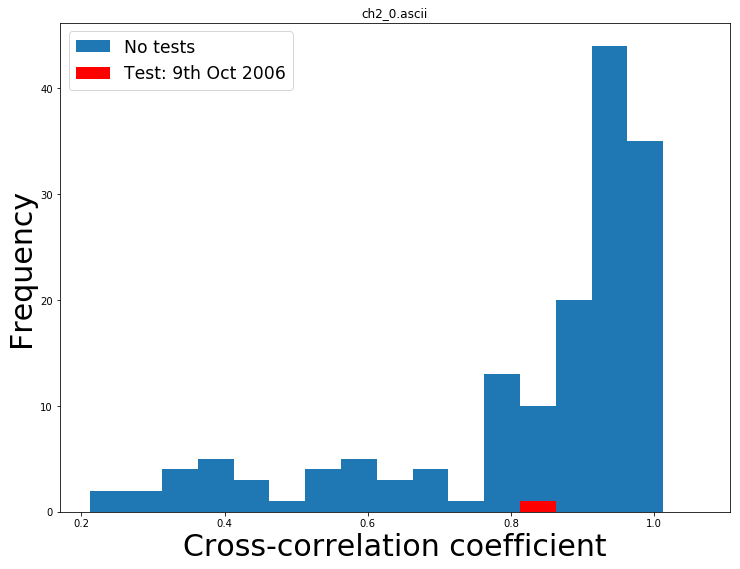
\includegraphics[width = 1.75in]{6ns54_0.png}} 
 	\subfloat[channel 1]{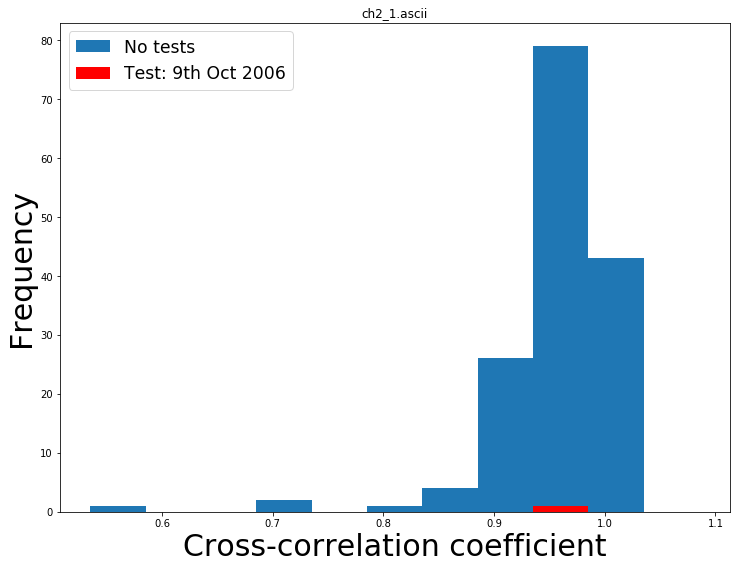
\includegraphics[width = 1.75in]{6ns54_1.png}}\\
 	\subfloat[channel 3]{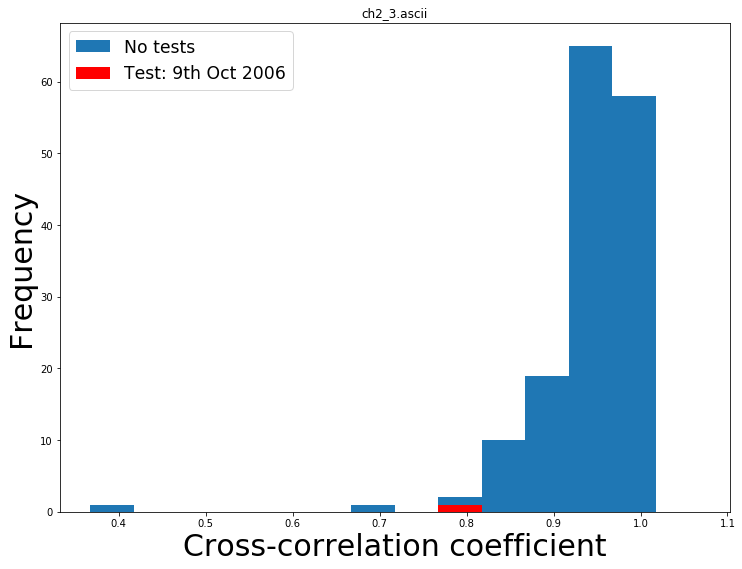
\includegraphics[width = 1.75in]{6ns54_3.png}}
 	\subfloat[channel 4]{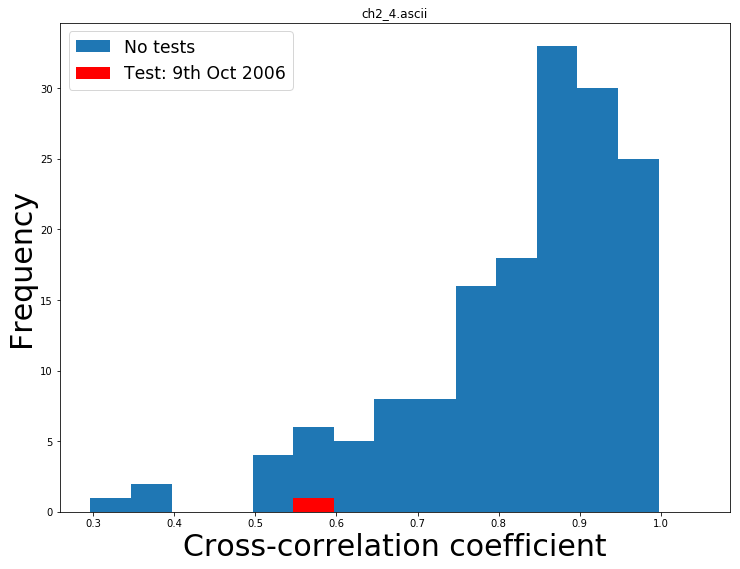
\includegraphics[width = 1.75in]{6ns54_4.png}}\\
 	\subfloat[channel 5]{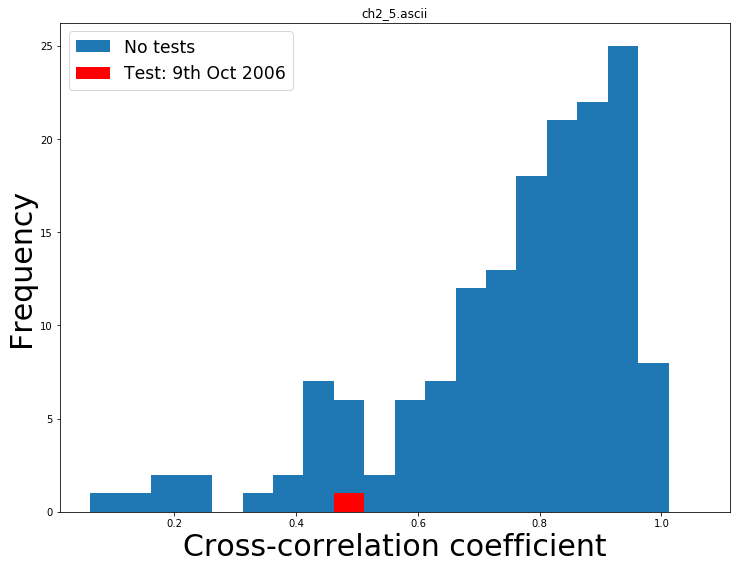
\includegraphics[width = 1.75in]{6ns54_5.png}}
 	\subfloat[channel 6]{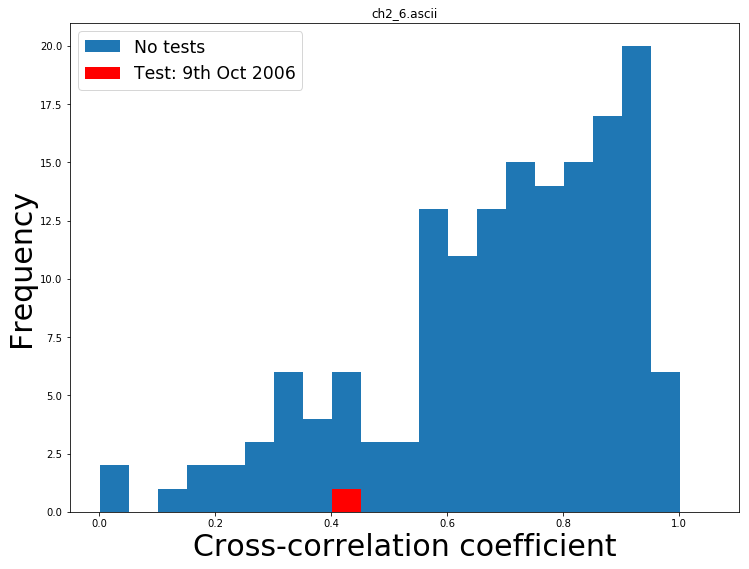
\includegraphics[width = 1.75in]{6ns54_6.png}}\\
 	\subfloat[channel 7]{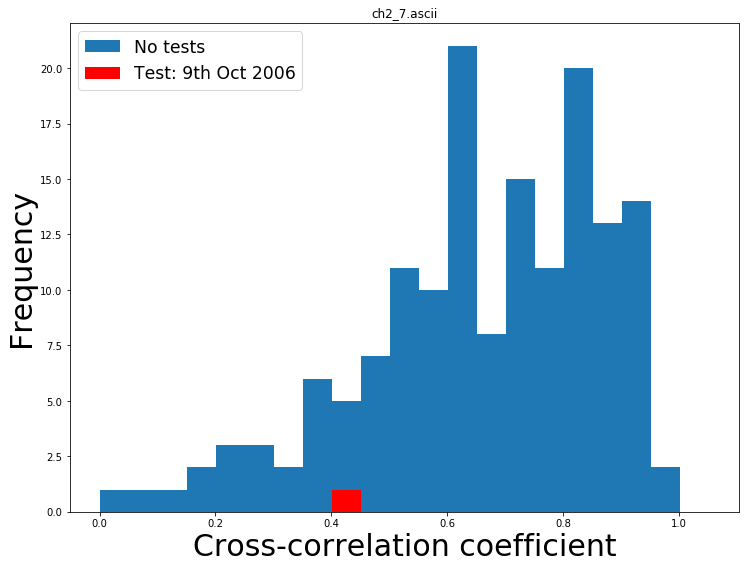
\includegraphics[width = 1.75in]{6ns54_7.png}}
 	\subfloat[channel 8]{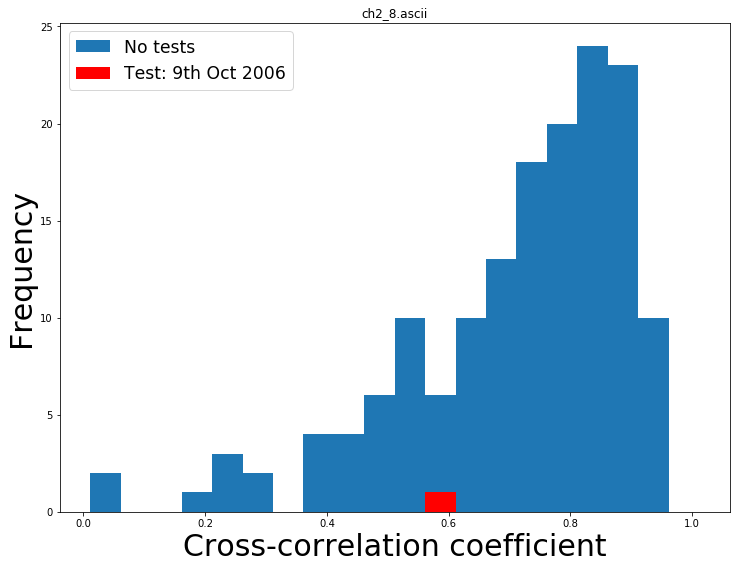
\includegraphics[width = 1.75in]{6ns54_8.png}}\\
 	\subfloat[channel 9]{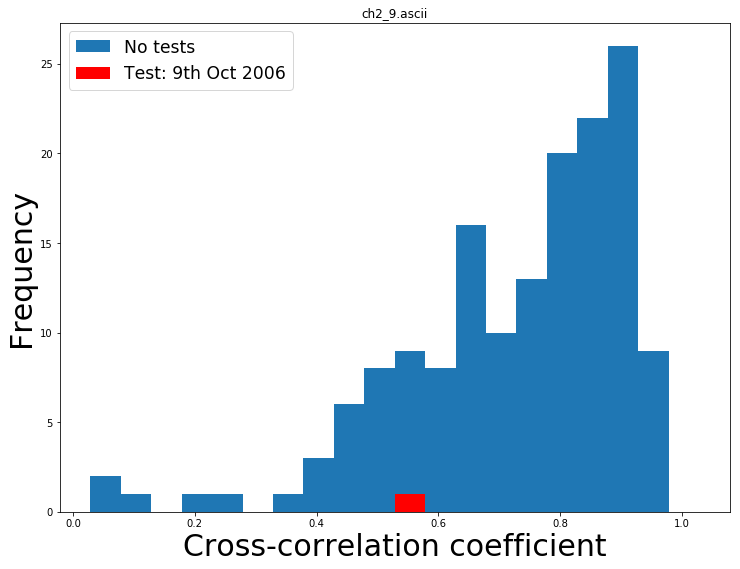
\includegraphics[width = 1.75in]{6ns54_9.png}}
 	\subfloat[channel 10]{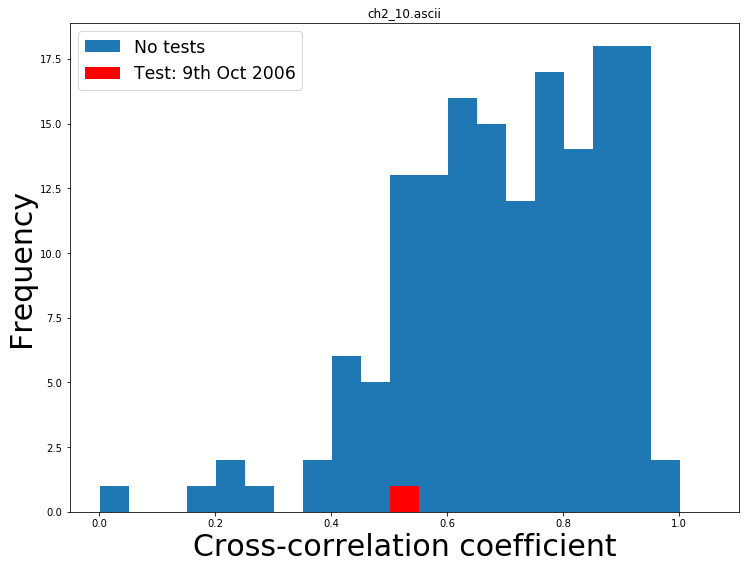
\includegraphics[width = 1.75in]{6ns54_10.png}}
 	\caption{Normalised cross--correlation coefficients of channel 2 for October 2006 test -- satellite ns54.}
 	\label{6ns54}
 \end{figure}
 
  \begin{figure}
 	\subfloat[channel 0]{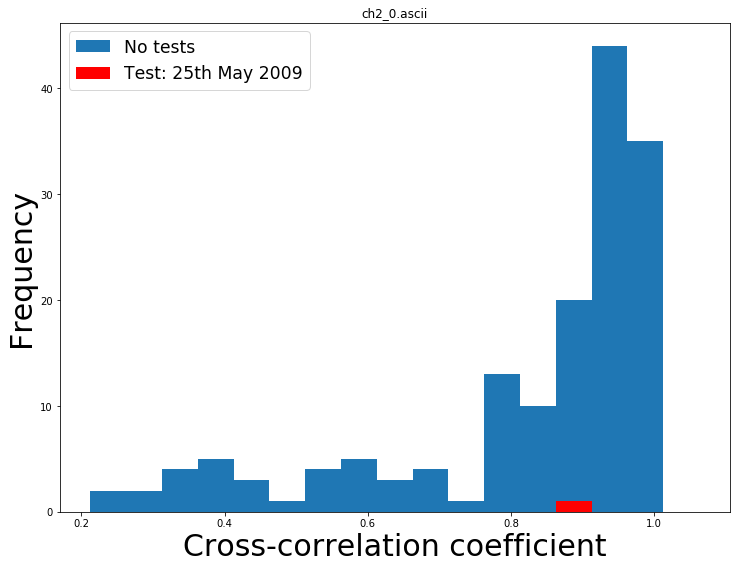
\includegraphics[width = 1.75in]{9ns54_0.png}} 
 	\subfloat[channel 1]{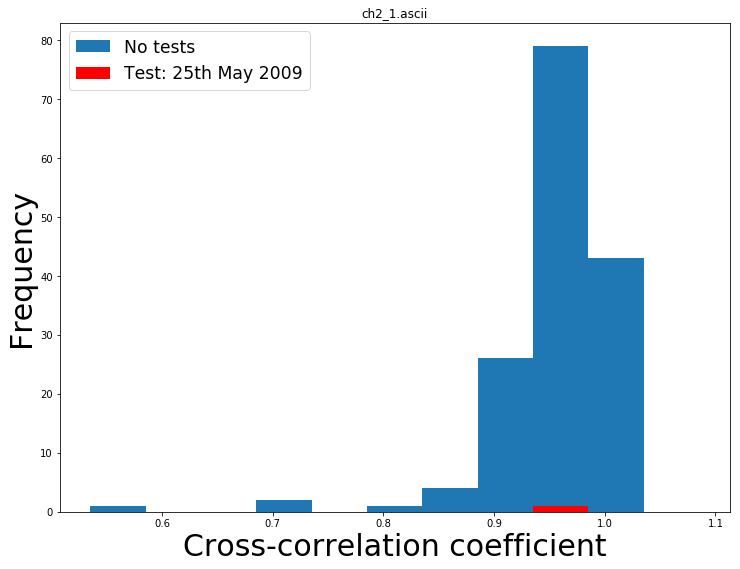
\includegraphics[width = 1.75in]{9ns54_1.png}}\\
 	\subfloat[channel 3]{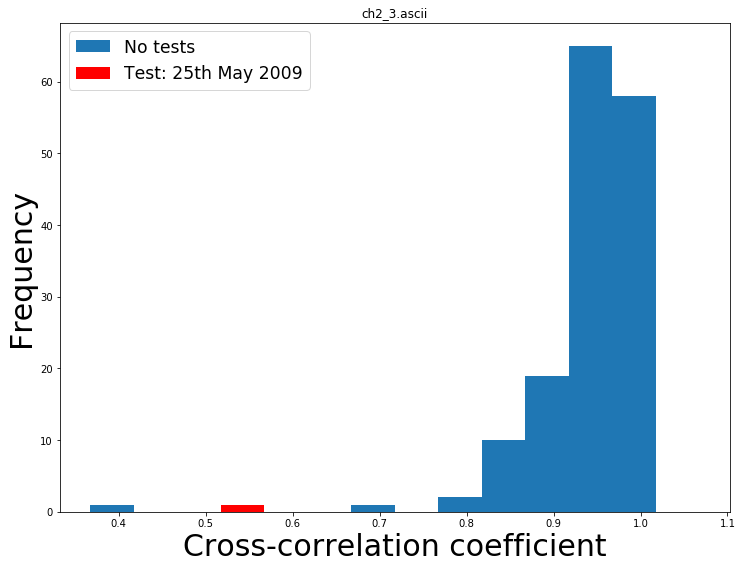
\includegraphics[width = 1.75in]{9ns54_3.png}}
 	\subfloat[channel 4]{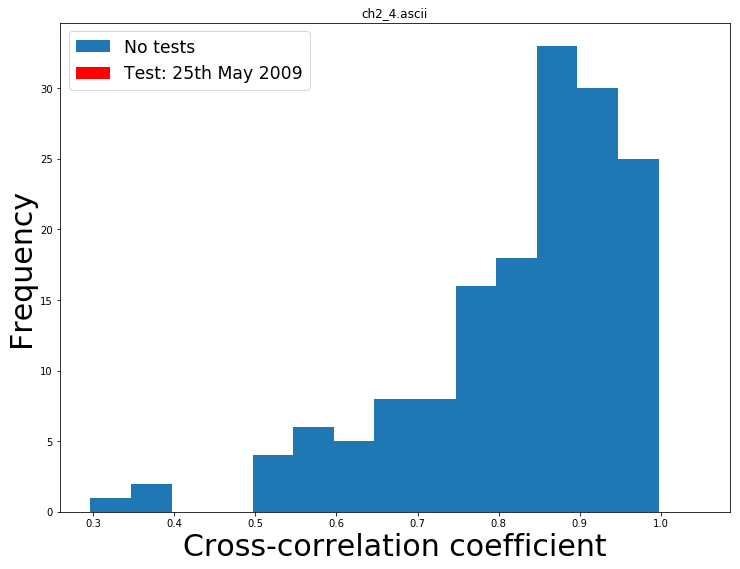
\includegraphics[width = 1.75in]{9ns54_4.png}}\\
 	\subfloat[channel 5]{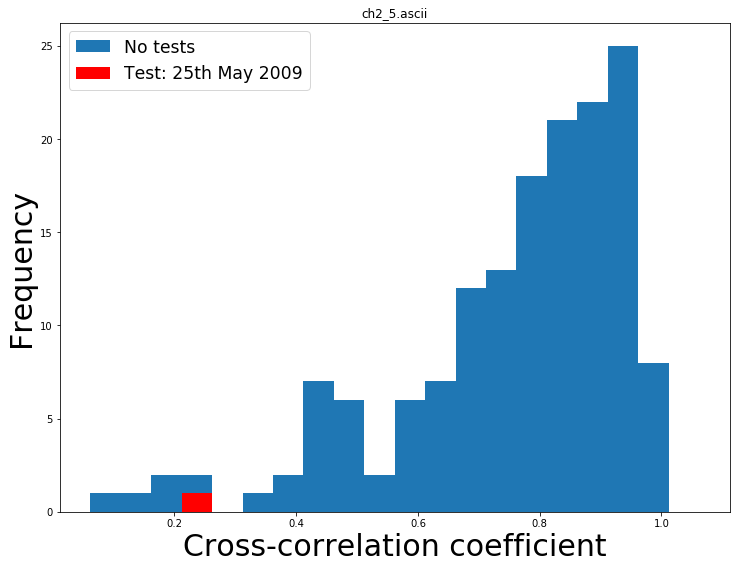
\includegraphics[width = 1.75in]{9ns54_5.png}}
 	\subfloat[channel 6]{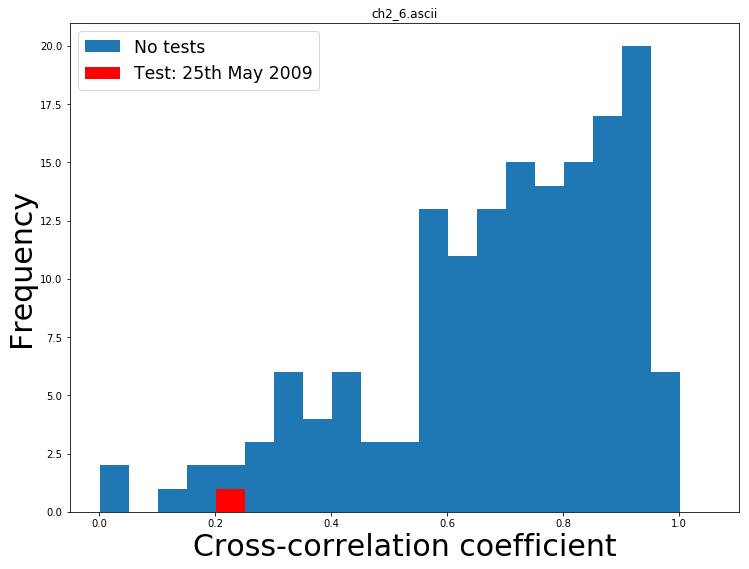
\includegraphics[width = 1.75in]{9ns54_6.png}}\\
 	\subfloat[channel 7]{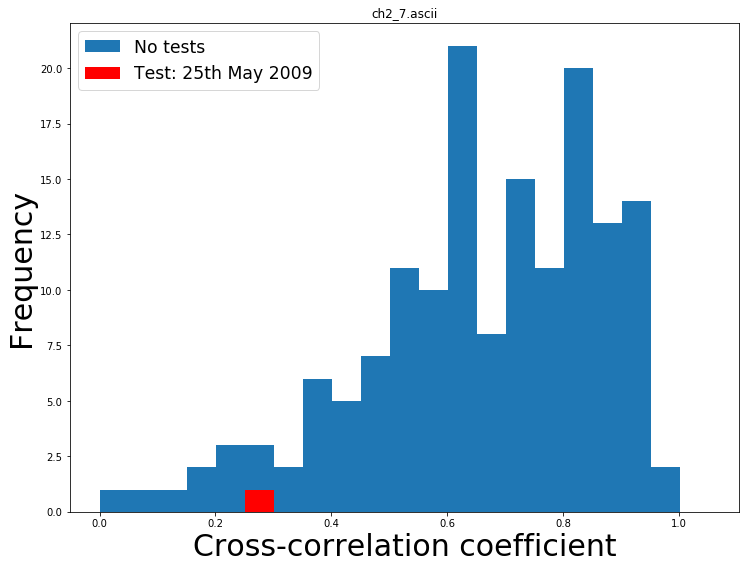
\includegraphics[width = 1.75in]{9ns54_7.png}}
 	\subfloat[channel 8]{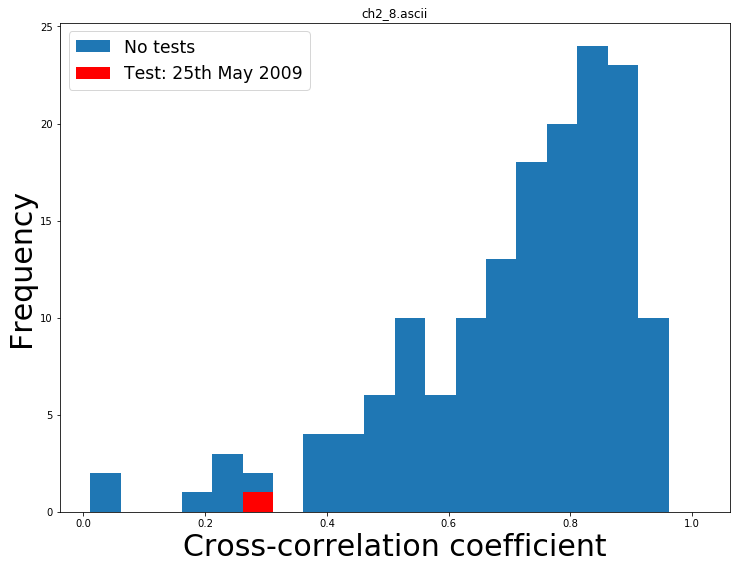
\includegraphics[width = 1.75in]{9ns54_8.png}}\\
 	\subfloat[channel 9]{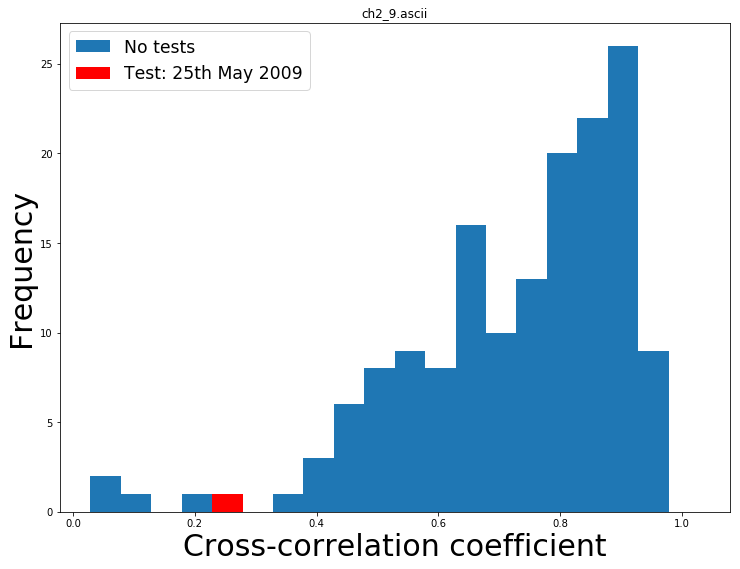
\includegraphics[width = 1.75in]{9ns54_9.png}}
 	\subfloat[channel 10]{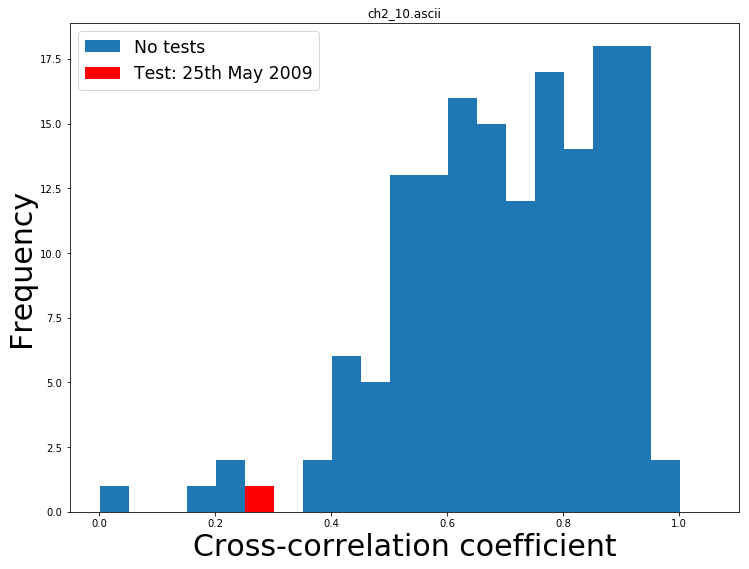
\includegraphics[width = 1.75in]{9ns54_10.png}}
 	\caption{Normalised cross--correlation coefficients of channel 2 for May 2009 test -- satellite ns54.}
 	\label{9ns54}
 \end{figure}

 \begin{figure}
	\subfloat[channel 0]{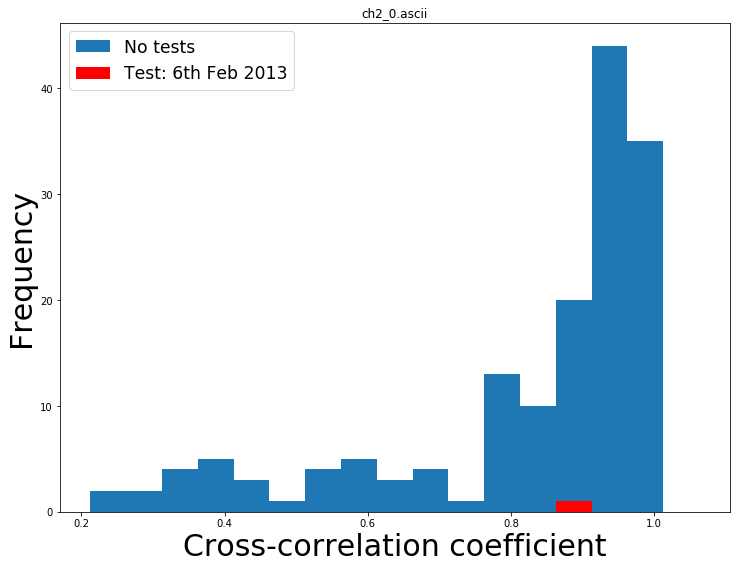
\includegraphics[width = 1.75in]{13ns54_0.png}} 
	\subfloat[channel 1]{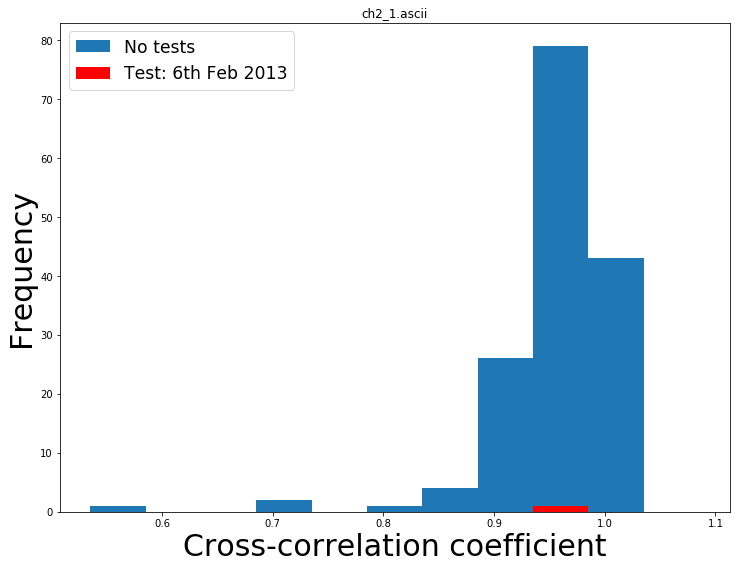
\includegraphics[width = 1.75in]{13ns54_1.png}}\\
	\subfloat[channel 3]{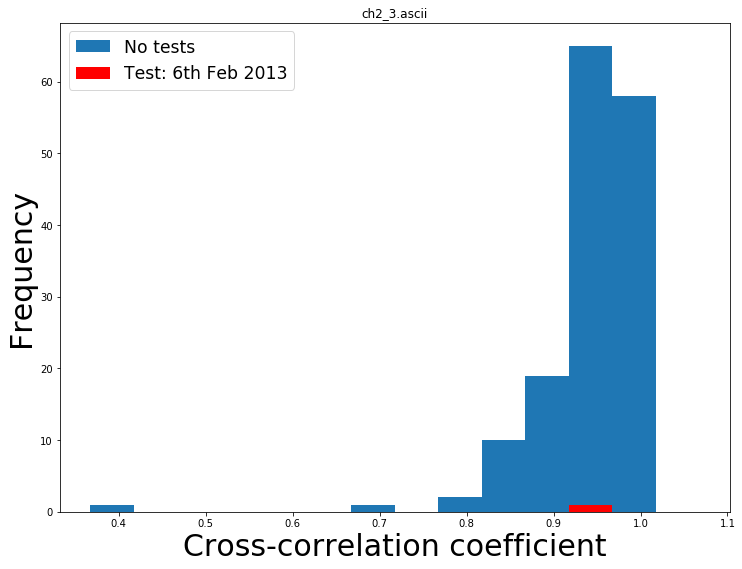
\includegraphics[width = 1.75in]{13ns54_3.png}}
	\subfloat[channel 4]{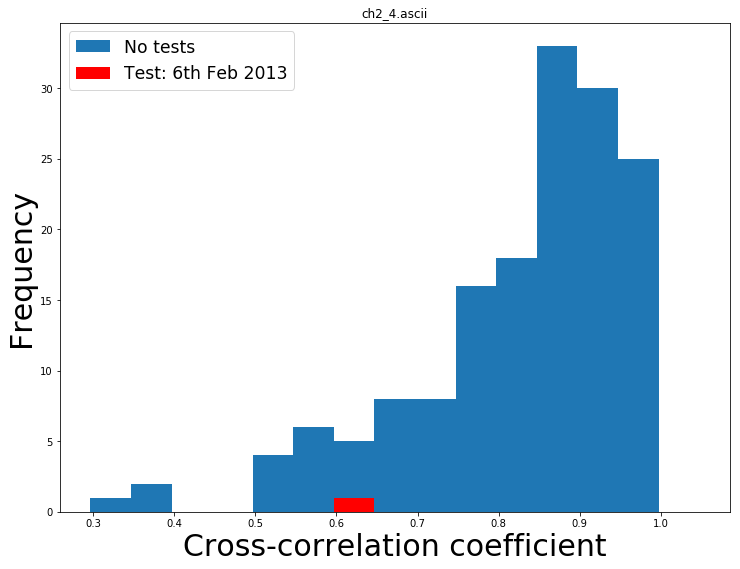
\includegraphics[width = 1.75in]{13ns54_4.png}}\\
	\subfloat[channel 5]{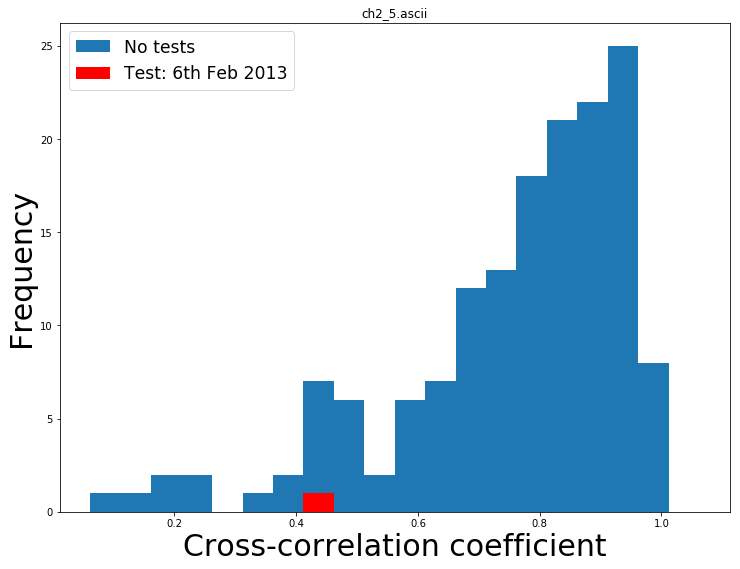
\includegraphics[width = 1.75in]{13ns54_5.png}}
	\subfloat[channel 6]{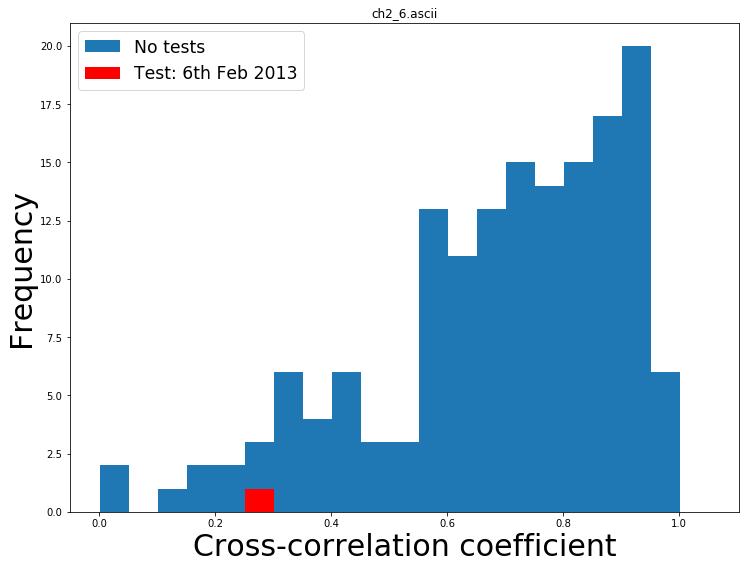
\includegraphics[width = 1.75in]{13ns54_6.png}}\\
	\subfloat[channel 7]{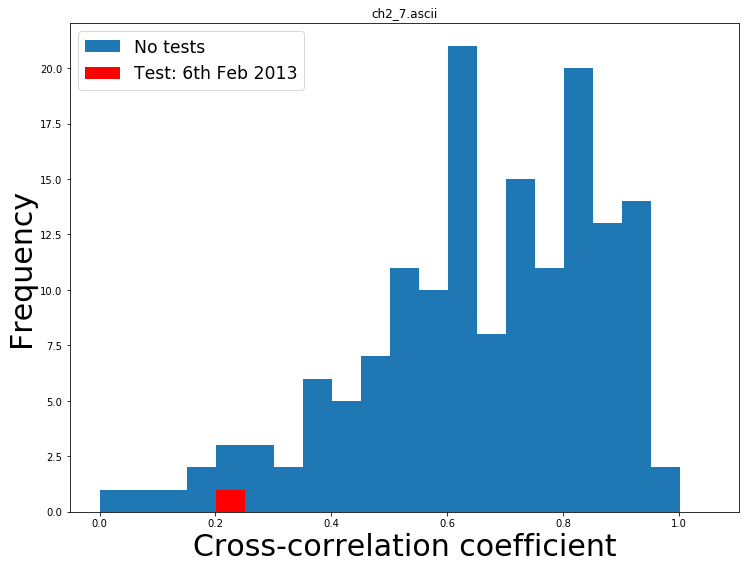
\includegraphics[width = 1.75in]{13ns54_7.png}}
	\subfloat[channel 8]{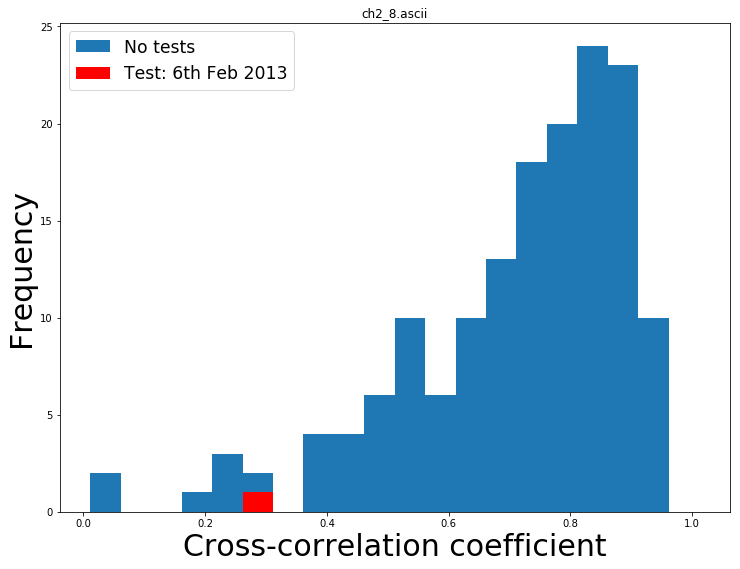
\includegraphics[width = 1.75in]{13ns54_8.png}}\\
	\subfloat[channel 9]{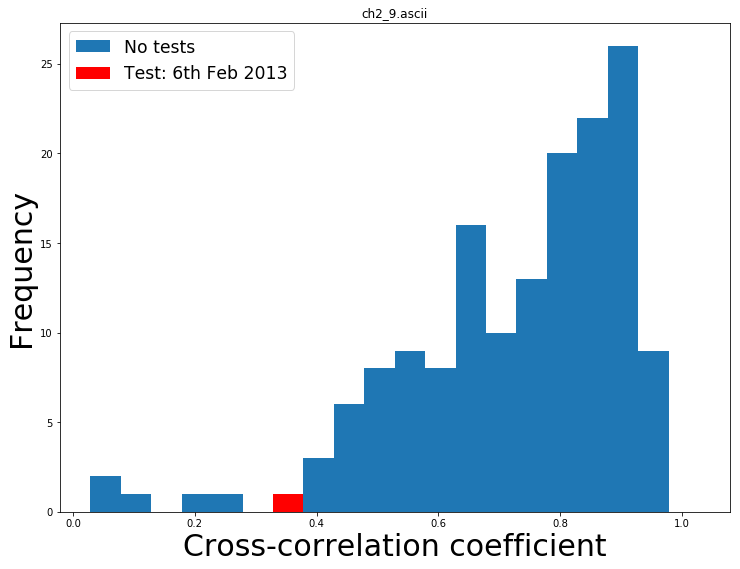
\includegraphics[width = 1.75in]{13ns54_9.png}}
	\subfloat[channel 10]{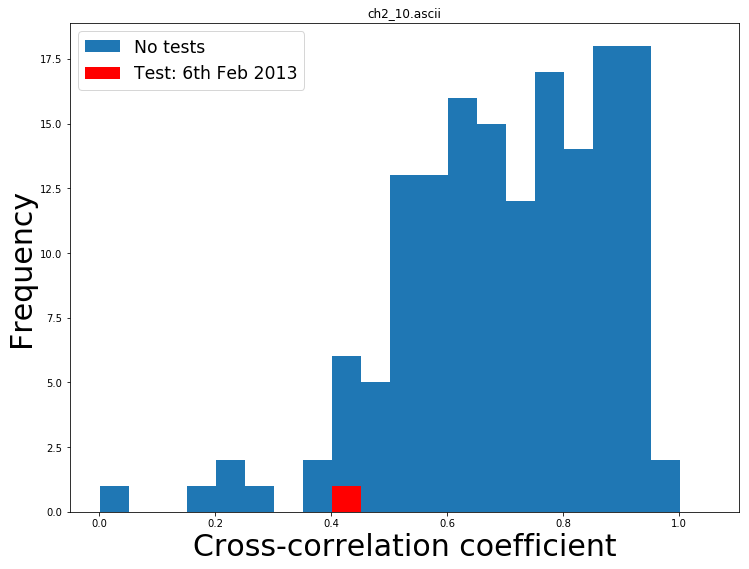
\includegraphics[width = 1.75in]{13ns54_10.png}}
	\caption{Normalised cross--correlation coefficients of channel 2 for February 2013 test -- satellite ns54.}
	\label{13ns54}
\end{figure}

 \begin{figure}
	\subfloat[channel 0]{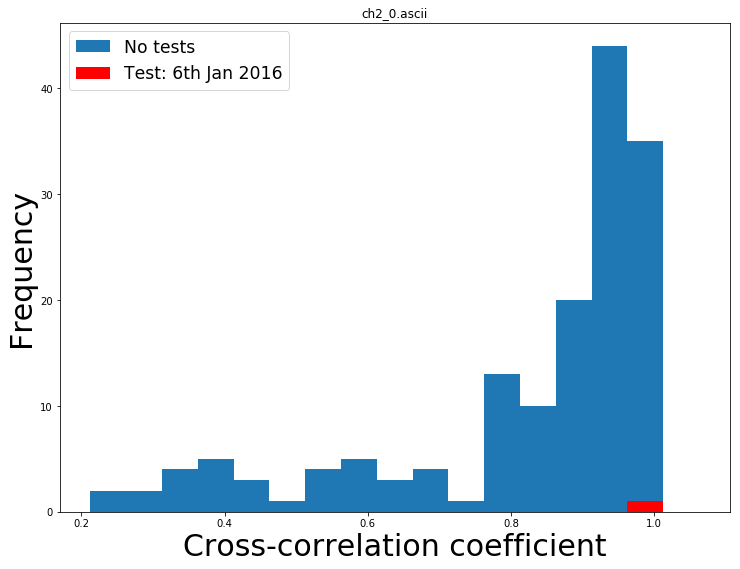
\includegraphics[width = 1.75in]{j16ns54_0.png}} 
	\subfloat[channel 1]{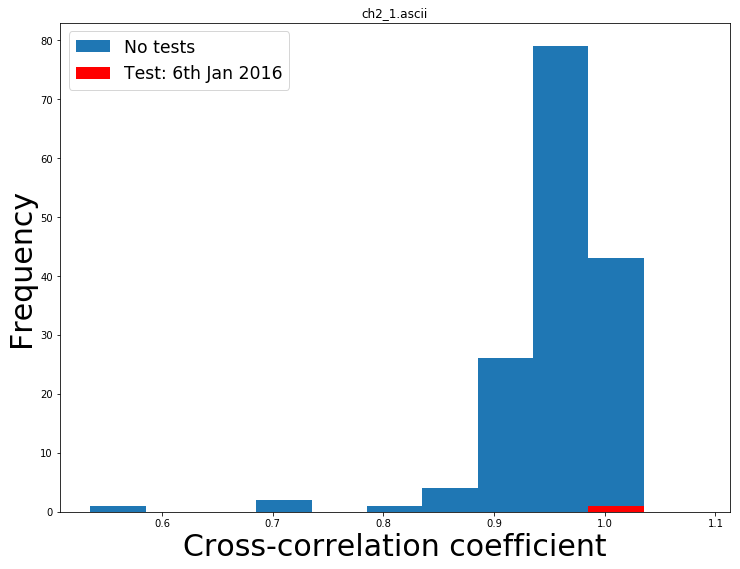
\includegraphics[width = 1.75in]{j16ns54_1.png}}\\
	\subfloat[channel 3]{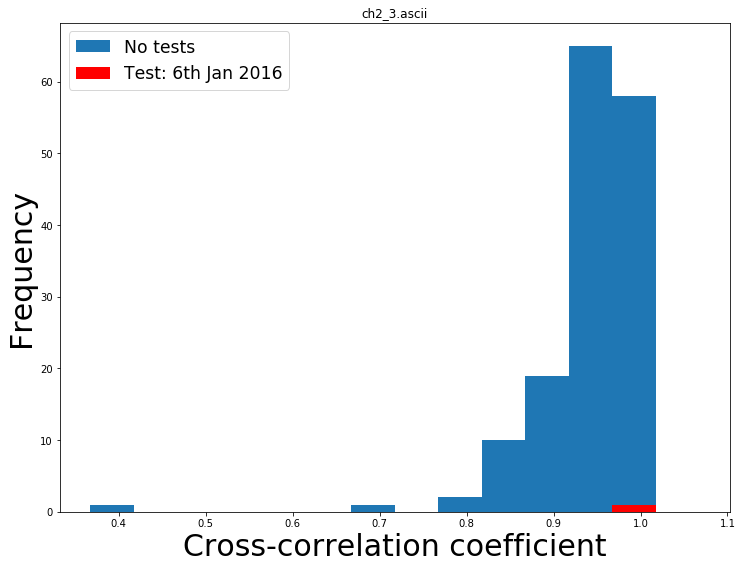
\includegraphics[width = 1.75in]{j16ns54_3.png}}
	\subfloat[channel 4]{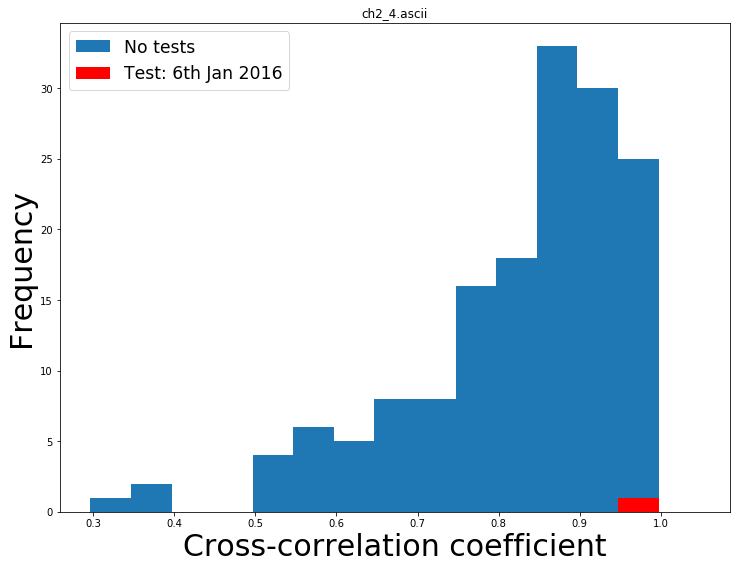
\includegraphics[width = 1.75in]{j16ns54_4.png}}\\
	\subfloat[channel 5]{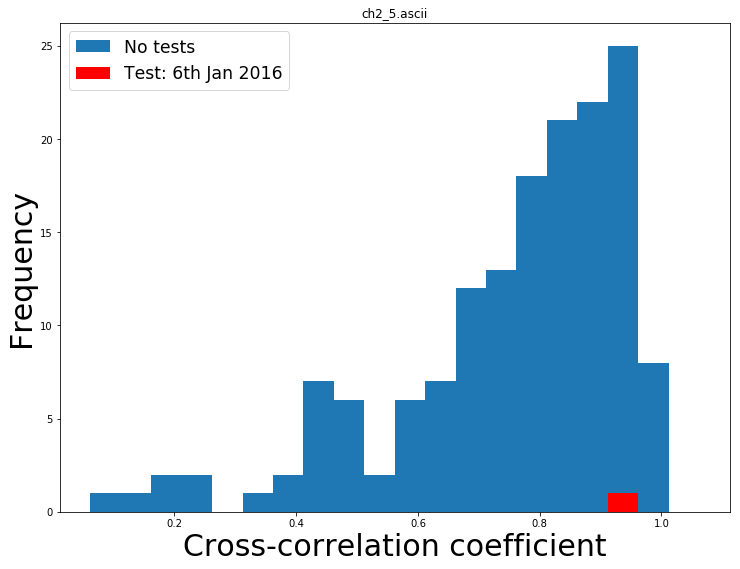
\includegraphics[width = 1.75in]{j16ns54_5.png}}
	\subfloat[channel 6]{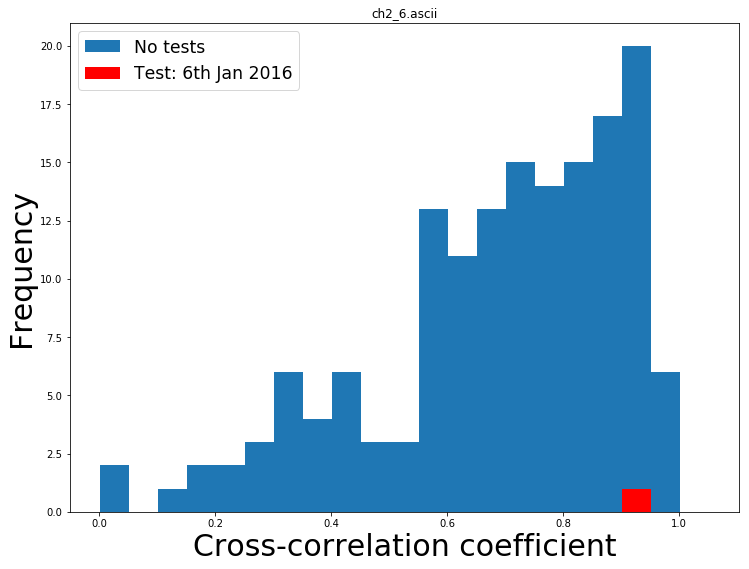
\includegraphics[width = 1.75in]{j16ns54_6.png}}\\
	\subfloat[channel 7]{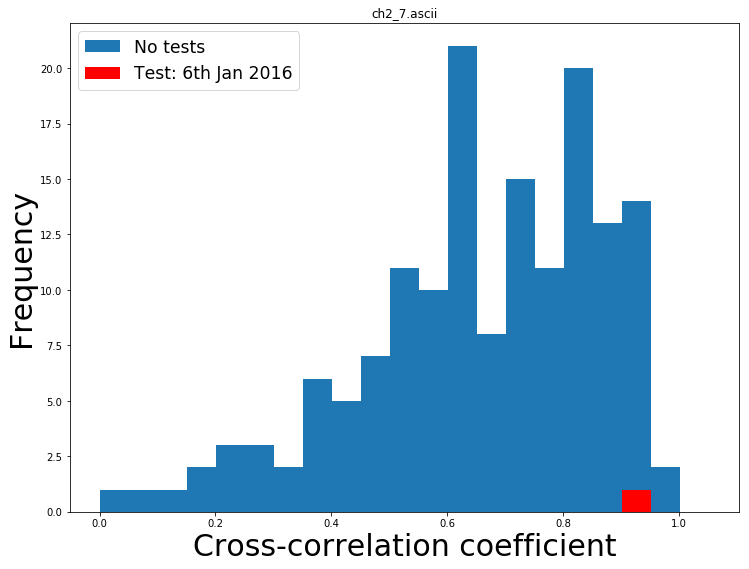
\includegraphics[width = 1.75in]{j16ns54_7.png}}
	\subfloat[channel 8]{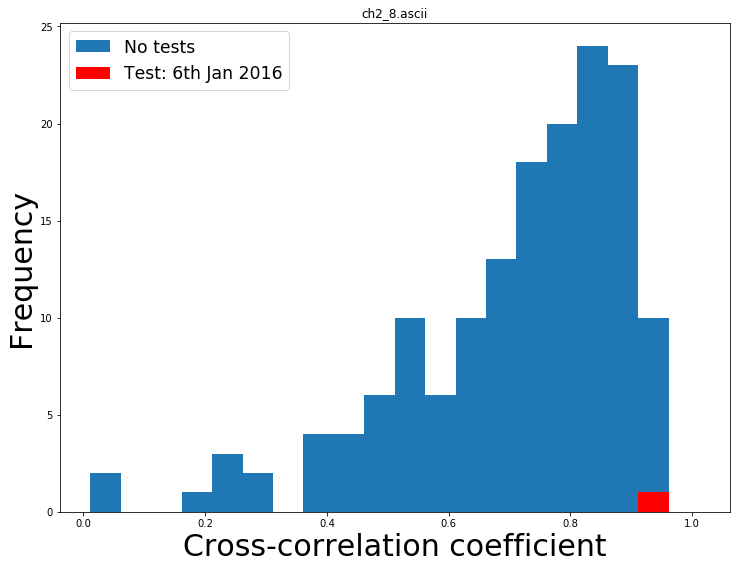
\includegraphics[width = 1.75in]{j16ns54_8.png}}\\
	\subfloat[channel 9]{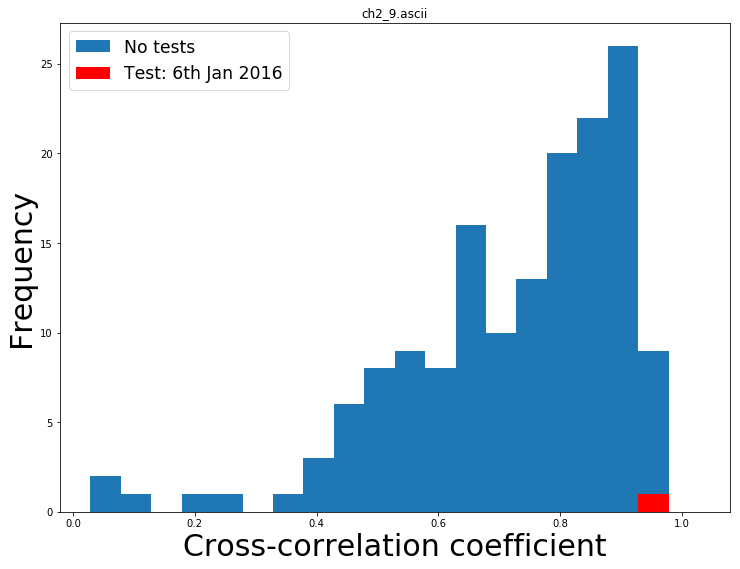
\includegraphics[width = 1.75in]{j16ns54_9.png}}
	\subfloat[channel 10]{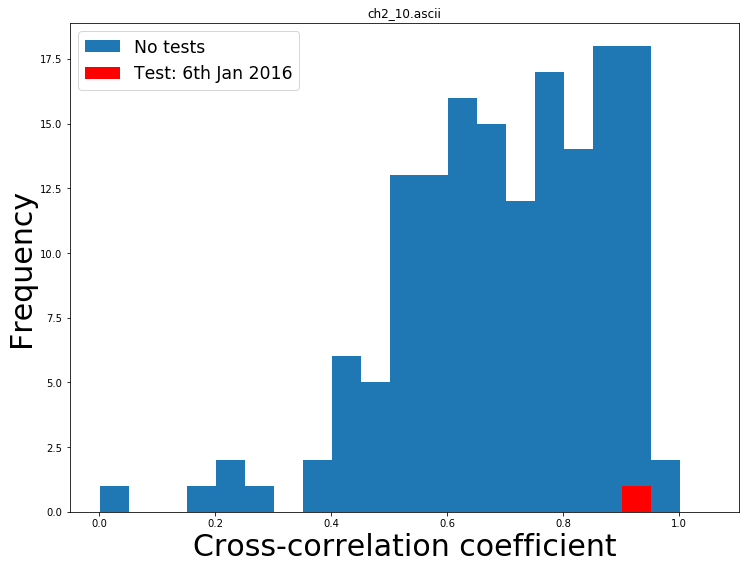
\includegraphics[width = 1.75in]{j16ns54_10.png}}
	\caption{Normalised cross--correlation coefficients of channel 2 for January 2016 test -- satellite ns54.}
	\label{j16ns54}
\end{figure}


\begin{figure}
	\subfloat[channel 0]{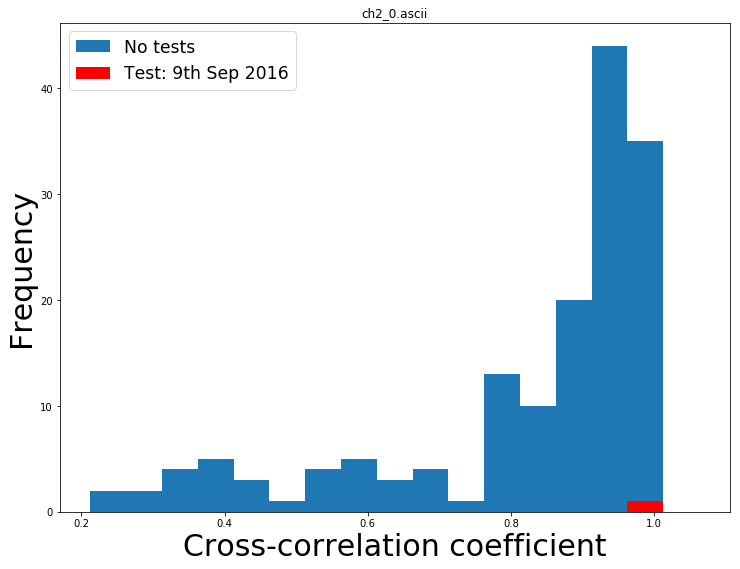
\includegraphics[width = 1.75in]{s16ns54_0.png}} 
	\subfloat[channel 1]{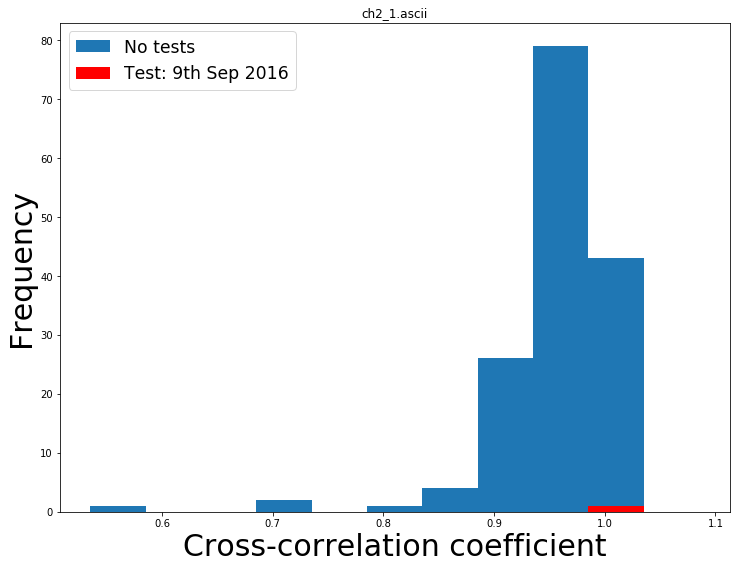
\includegraphics[width = 1.75in]{s16ns54_1.png}}\\
	\subfloat[channel 3]{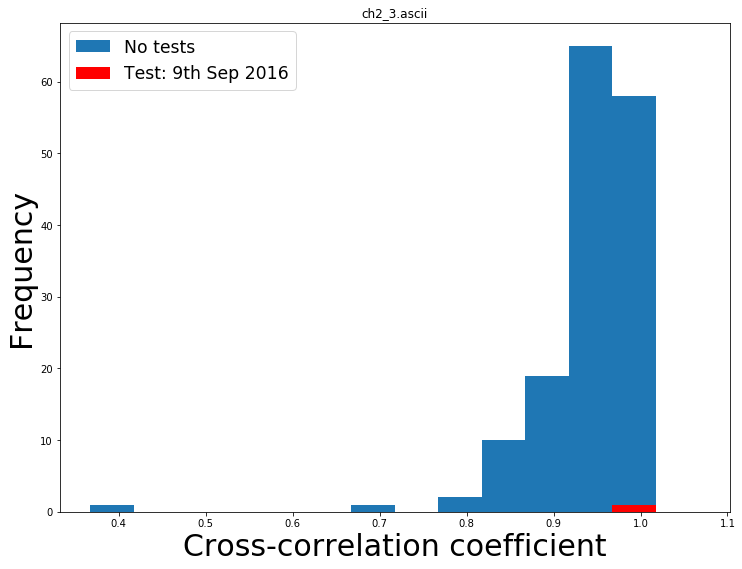
\includegraphics[width = 1.75in]{s16ns54_3.png}}
	\subfloat[channel 4]{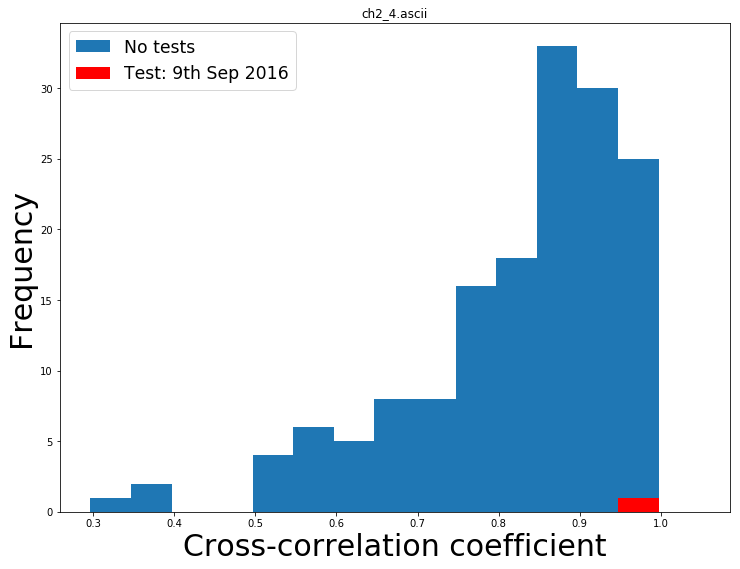
\includegraphics[width = 1.75in]{s16ns54_4.png}}\\
	\subfloat[channel 5]{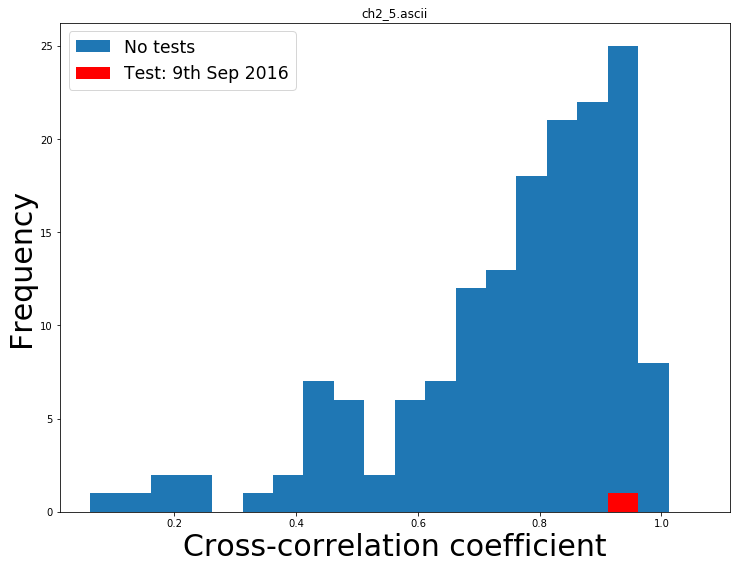
\includegraphics[width = 1.75in]{s16ns54_5.png}}
	\subfloat[channel 6]{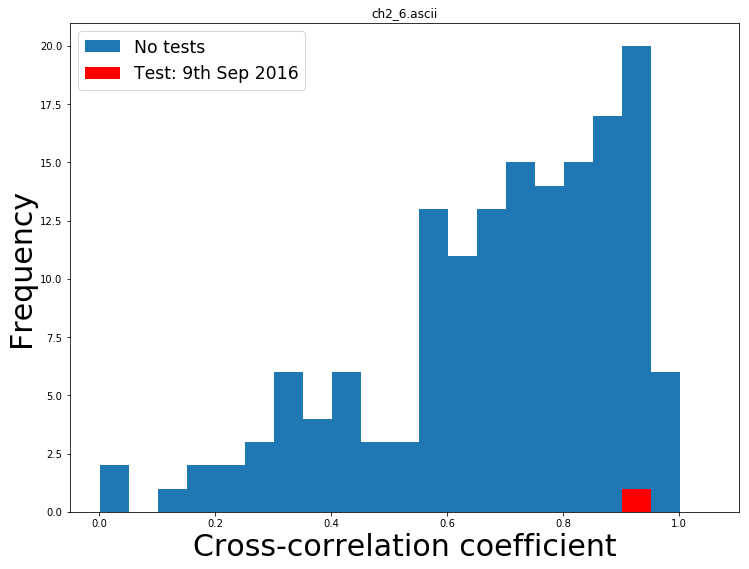
\includegraphics[width = 1.75in]{s16ns54_6.png}}\\
	\subfloat[channel 7]{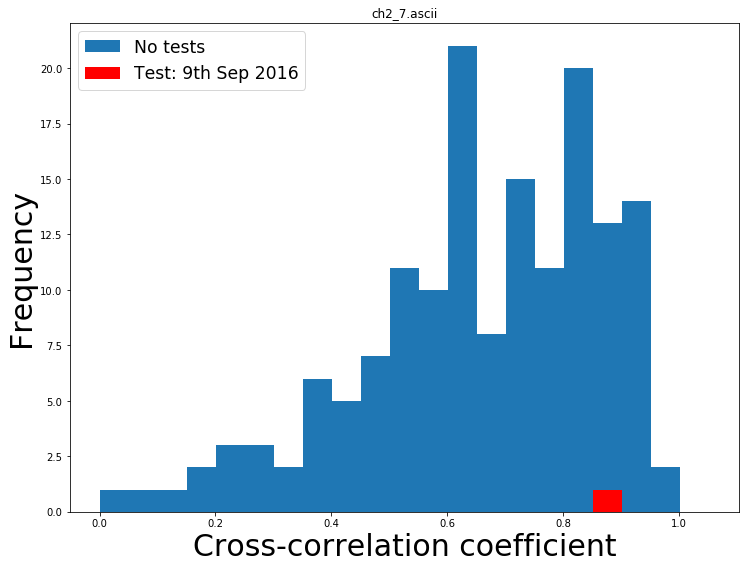
\includegraphics[width = 1.75in]{s16ns54_7.png}}
	\subfloat[channel 8]{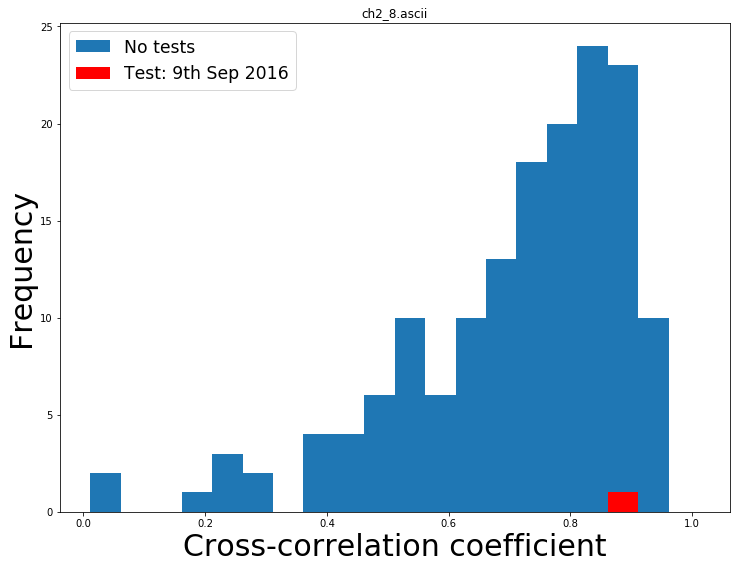
\includegraphics[width = 1.75in]{s16ns54_8.png}}\\
	\subfloat[channel 9]{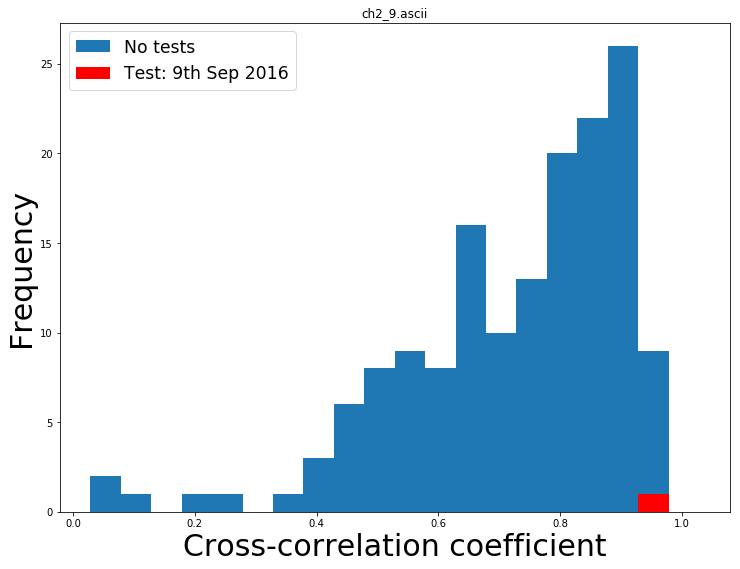
\includegraphics[width = 1.75in]{s16ns54_9.png}}
	\subfloat[channel 10]{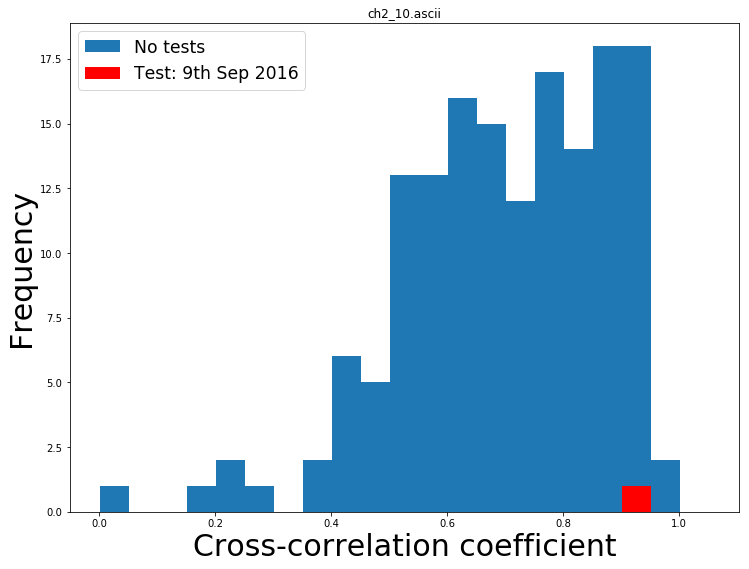
\includegraphics[width = 1.75in]{s16ns54_10.png}}
	\caption{Normalised cross--correlation coefficients of channel 2 for September 2016 test -- satellite ns54.}
	\label{s16ns54}
\end{figure}

 \begin{figure}
	\subfloat[channel 0]{\includegraphics[width = 1.75in]{6ns56_0.png}} 
	\subfloat[channel 1]{\includegraphics[width = 1.75in]{6ns56_1.png}}\\
	\subfloat[channel 3]{\includegraphics[width = 1.75in]{6ns56_3.png}}
	\subfloat[channel 4]{\includegraphics[width = 1.75in]{6ns56_4.png}}\\
	\subfloat[channel 5]{\includegraphics[width = 1.75in]{6ns56_5.png}}
	\subfloat[channel 6]{\includegraphics[width = 1.75in]{6ns56_6.png}}\\
	\subfloat[channel 7]{\includegraphics[width = 1.75in]{6ns56_7.png}}
	\subfloat[channel 8]{\includegraphics[width = 1.75in]{6ns56_8.png}}\\
	\subfloat[channel 9]{\includegraphics[width = 1.75in]{6ns56_9.png}}
	\subfloat[channel 10]{\includegraphics[width = 1.75in]{6ns56_10.png}}
	\caption{Normalised cross--correlation coefficients of channel 2 for October 2006 test -- satellite ns56.}
	\label{6ns56}
\end{figure}

  \begin{figure}
	\subfloat[channel 0]{\includegraphics[width = 1.75in]{9ns56_0.png}} 
	\subfloat[channel 1]{\includegraphics[width = 1.75in]{9ns56_1.png}}\\
	\subfloat[channel 3]{\includegraphics[width = 1.75in]{9ns56_3.png}}
	\subfloat[channel 4]{\includegraphics[width = 1.75in]{9ns56_4.png}}\\
	\subfloat[channel 5]{\includegraphics[width = 1.75in]{9ns56_5.png}}
	\subfloat[channel 6]{\includegraphics[width = 1.75in]{9ns56_6.png}}\\
	\subfloat[channel 7]{\includegraphics[width = 1.75in]{9ns56_7.png}}
	\subfloat[channel 8]{\includegraphics[width = 1.75in]{9ns56_8.png}}\\
	\subfloat[channel 9]{\includegraphics[width = 1.75in]{9ns56_9.png}}
	\subfloat[channel 10]{\includegraphics[width = 1.75in]{9ns56_10.png}}
	\caption{Normalised cross--correlation coefficients of channel 2 for May 2009 test -- satellite ns56.}
	\label{9ns56}
\end{figure}

\begin{figure}
	\subfloat[channel 0]{\includegraphics[width = 1.75in]{13ns56_0.png}} 
	\subfloat[channel 1]{\includegraphics[width = 1.75in]{13ns56_1.png}}\\
	\subfloat[channel 3]{\includegraphics[width = 1.75in]{13ns56_3.png}}
	\subfloat[channel 4]{\includegraphics[width = 1.75in]{13ns56_4.png}}\\
	\subfloat[channel 5]{\includegraphics[width = 1.75in]{13ns56_5.png}}
	\subfloat[channel 6]{\includegraphics[width = 1.75in]{13ns56_6.png}}\\
	\subfloat[channel 7]{\includegraphics[width = 1.75in]{13ns56_7.png}}
	\subfloat[channel 8]{\includegraphics[width = 1.75in]{13ns56_8.png}}\\
	\subfloat[channel 9]{\includegraphics[width = 1.75in]{13ns56_9.png}}
	\subfloat[channel 10]{\includegraphics[width = 1.75in]{13ns56_10.png}}
	\caption{Normalised cross--correlation coefficients of channel 2 for February 2013 test -- satellite ns56.}
	\label{13ns56}
\end{figure}

\begin{figure}
	\subfloat[channel 0]{\includegraphics[width = 1.75in]{j16ns56_0.png}} 
	\subfloat[channel 1]{\includegraphics[width = 1.75in]{j16ns56_1.png}}\\
	\subfloat[channel 3]{\includegraphics[width = 1.75in]{j16ns56_3.png}}
	\subfloat[channel 4]{\includegraphics[width = 1.75in]{j16ns56_4.png}}\\
	\subfloat[channel 5]{\includegraphics[width = 1.75in]{j16ns56_5.png}}
	\subfloat[channel 6]{\includegraphics[width = 1.75in]{j16ns56_6.png}}\\
	\subfloat[channel 7]{\includegraphics[width = 1.75in]{j16ns56_7.png}}
	\subfloat[channel 8]{\includegraphics[width = 1.75in]{j16ns56_8.png}}\\
	\subfloat[channel 9]{\includegraphics[width = 1.75in]{j16ns56_9.png}}
	\subfloat[channel 10]{\includegraphics[width = 1.75in]{j16ns56_10.png}}
	\caption{Normalised cross--correlation coefficients of channel 2 for January 2016 test -- satellite ns56.}
	\label{j16ns56}
\end{figure}


\begin{figure}
	\subfloat[channel 0]{\includegraphics[width = 1.75in]{s16ns56_0.png}} 
	\subfloat[channel 1]{\includegraphics[width = 1.75in]{s16ns56_1.png}}\\
	\subfloat[channel 3]{\includegraphics[width = 1.75in]{s16ns56_3.png}}
	\subfloat[channel 4]{\includegraphics[width = 1.75in]{s16ns56_4.png}}\\
	\subfloat[channel 5]{\includegraphics[width = 1.75in]{s16ns56_5.png}}
	\subfloat[channel 6]{\includegraphics[width = 1.75in]{s16ns56_6.png}}\\
	\subfloat[channel 7]{\includegraphics[width = 1.75in]{s16ns56_7.png}}
	\subfloat[channel 8]{\includegraphics[width = 1.75in]{s16ns56_8.png}}\\
	\subfloat[channel 9]{\includegraphics[width = 1.75in]{s16ns56_9.png}}
	\subfloat[channel 10]{\includegraphics[width = 1.75in]{s16ns56_10.png}}
	\caption{Normalised cross--correlation coefficients of channel 2 for September 2016 test -- satellite ns56.}
	\label{s16ns56}
\end{figure}


\begin{figure}
	\subfloat[channel 0]{\includegraphics[width = 1.75in]{6ns59_0.png}} 
	\subfloat[channel 1]{\includegraphics[width = 1.75in]{6ns59_1.png}}\\
	\subfloat[channel 3]{\includegraphics[width = 1.75in]{6ns59_3.png}}
	\subfloat[channel 4]{\includegraphics[width = 1.75in]{6ns59_4.png}}\\
	\subfloat[channel 5]{\includegraphics[width = 1.75in]{6ns59_5.png}}
	\subfloat[channel 6]{\includegraphics[width = 1.75in]{6ns59_6.png}}\\
	\subfloat[channel 7]{\includegraphics[width = 1.75in]{6ns59_7.png}}
	\subfloat[channel 8]{\includegraphics[width = 1.75in]{6ns59_8.png}}\\
	\subfloat[channel 9]{\includegraphics[width = 1.75in]{6ns59_9.png}}
	\subfloat[channel 10]{\includegraphics[width = 1.75in]{6ns59_10.png}}
	\caption{Normalised cross--correlation coefficients of channel 2 for October 2006 test -- satellite ns59.}
	\label{6ns59}
\end{figure}

\begin{figure}
	\subfloat[channel 0]{\includegraphics[width = 1.75in]{9ns59_0.png}} 
	\subfloat[channel 1]{\includegraphics[width = 1.75in]{9ns59_1.png}}\\
	\subfloat[channel 3]{\includegraphics[width = 1.75in]{9ns59_3.png}}
	\subfloat[channel 4]{\includegraphics[width = 1.75in]{9ns59_4.png}}\\
	\subfloat[channel 5]{\includegraphics[width = 1.75in]{9ns59_5.png}}
	\subfloat[channel 6]{\includegraphics[width = 1.75in]{9ns59_6.png}}\\
	\subfloat[channel 7]{\includegraphics[width = 1.75in]{9ns59_7.png}}
	\subfloat[channel 8]{\includegraphics[width = 1.75in]{9ns59_8.png}}\\
	\subfloat[channel 9]{\includegraphics[width = 1.75in]{9ns59_9.png}}
	\subfloat[channel 10]{\includegraphics[width = 1.75in]{9ns59_10.png}}
	\caption{Normalised cross--correlation coefficients of channel 2 for May 2009 test -- satellite ns59.}
	\label{9ns59}
\end{figure}

\begin{figure}
	\subfloat[channel 0]{\includegraphics[width = 1.75in]{13ns59_0.png}} 
	\subfloat[channel 1]{\includegraphics[width = 1.75in]{13ns59_1.png}}\\
	\subfloat[channel 3]{\includegraphics[width = 1.75in]{13ns59_3.png}}
	\subfloat[channel 4]{\includegraphics[width = 1.75in]{13ns59_4.png}}\\
	\subfloat[channel 5]{\includegraphics[width = 1.75in]{13ns59_5.png}}
	\subfloat[channel 6]{\includegraphics[width = 1.75in]{13ns59_6.png}}\\
	\subfloat[channel 7]{\includegraphics[width = 1.75in]{13ns59_7.png}}
	\subfloat[channel 8]{\includegraphics[width = 1.75in]{13ns59_8.png}}\\
	\subfloat[channel 9]{\includegraphics[width = 1.75in]{13ns59_9.png}}
	\subfloat[channel 10]{\includegraphics[width = 1.75in]{13ns59_10.png}}
	\caption{Normalised cross--correlation coefficients of channel 2 for February 2013 test -- satellite ns59.}
	\label{13ns59}
\end{figure}

\begin{figure}
	\subfloat[channel 0]{\includegraphics[width = 1.75in]{j16ns59_0.png}} 
	\subfloat[channel 1]{\includegraphics[width = 1.75in]{j16ns59_1.png}}\\
	\subfloat[channel 3]{\includegraphics[width = 1.75in]{j16ns59_3.png}}
	\subfloat[channel 4]{\includegraphics[width = 1.75in]{j16ns59_4.png}}\\
	\subfloat[channel 5]{\includegraphics[width = 1.75in]{j16ns59_5.png}}
	\subfloat[channel 6]{\includegraphics[width = 1.75in]{j16ns59_6.png}}\\
	\subfloat[channel 7]{\includegraphics[width = 1.75in]{j16ns59_7.png}}
	\subfloat[channel 8]{\includegraphics[width = 1.75in]{j16ns59_8.png}}\\
	\subfloat[channel 9]{\includegraphics[width = 1.75in]{j16ns59_9.png}}
	\subfloat[channel 10]{\includegraphics[width = 1.75in]{j16ns59_10.png}}
	\caption{Normalised cross--correlation coefficients of channel 2 for January 2016 test -- satellite ns59.}
	\label{j16ns59}
\end{figure}


\begin{figure}
	\subfloat[channel 0]{\includegraphics[width = 1.75in]{s16ns59_0.png}} 
	\subfloat[channel 1]{\includegraphics[width = 1.75in]{s16ns59_1.png}}\\
	\subfloat[channel 3]{\includegraphics[width = 1.75in]{s16ns59_3.png}}
	\subfloat[channel 4]{\includegraphics[width = 1.75in]{s16ns59_4.png}}\\
	\subfloat[channel 5]{\includegraphics[width = 1.75in]{s16ns59_5.png}}
	\subfloat[channel 6]{\includegraphics[width = 1.75in]{s16ns59_6.png}}\\
	\subfloat[channel 7]{\includegraphics[width = 1.75in]{s16ns59_7.png}}
	\subfloat[channel 8]{\includegraphics[width = 1.75in]{s16ns59_8.png}}\\
	\subfloat[channel 9]{\includegraphics[width = 1.75in]{s16ns59_9.png}}
	\subfloat[channel 10]{\includegraphics[width = 1.75in]{s16ns59_10.png}}
	\caption{Normalised cross--correlation coefficients of channel 2 for September 2016 test -- satellite ns59.}
	\label{s16ns59}
\end{figure}


\begin{figure}
	\subfloat[channel 0]{\includegraphics[width = 1.75in]{6ns60_0.png}} 
	\subfloat[channel 1]{\includegraphics[width = 1.75in]{6ns60_1.png}}\\
	\subfloat[channel 3]{\includegraphics[width = 1.75in]{6ns60_3.png}}
	\subfloat[channel 4]{\includegraphics[width = 1.75in]{6ns60_4.png}}\\
	\subfloat[channel 5]{\includegraphics[width = 1.75in]{6ns60_5.png}}
	\subfloat[channel 6]{\includegraphics[width = 1.75in]{6ns60_6.png}}\\
	\subfloat[channel 7]{\includegraphics[width = 1.75in]{6ns60_7.png}}
	\subfloat[channel 8]{\includegraphics[width = 1.75in]{6ns60_8.png}}\\
	\subfloat[channel 9]{\includegraphics[width = 1.75in]{6ns60_9.png}}
	\subfloat[channel 10]{\includegraphics[width = 1.75in]{6ns60_10.png}}
	\caption{Normalised cross--correlation coefficients of channel 2 for October 2006 test.}
	\label{6ns60}
\end{figure}

\begin{figure}
	\subfloat[channel 0]{\includegraphics[width = 1.75in]{9ns60_0.png}} 
	\subfloat[channel 1]{\includegraphics[width = 1.75in]{9ns60_1.png}}\\
	\subfloat[channel 3]{\includegraphics[width = 1.75in]{9ns60_3.png}}
	\subfloat[channel 4]{\includegraphics[width = 1.75in]{9ns60_4.png}}\\
	\subfloat[channel 5]{\includegraphics[width = 1.75in]{9ns60_5.png}}
	\subfloat[channel 6]{\includegraphics[width = 1.75in]{9ns60_6.png}}\\
	\subfloat[channel 7]{\includegraphics[width = 1.75in]{9ns60_7.png}}
	\subfloat[channel 8]{\includegraphics[width = 1.75in]{9ns60_8.png}}\\
	\subfloat[channel 9]{\includegraphics[width = 1.75in]{9ns60_9.png}}
	\subfloat[channel 10]{\includegraphics[width = 1.75in]{9ns60_10.png}}
	\caption{Normalised cross--correlation coefficients of channel 2 for May 2009 test -- satellite ns60.}
	\label{9ns60}
\end{figure}

\begin{figure}
	\subfloat[channel 0]{\includegraphics[width = 1.75in]{13ns60_0.png}} 
	\subfloat[channel 1]{\includegraphics[width = 1.75in]{13ns60_1.png}}\\
	\subfloat[channel 3]{\includegraphics[width = 1.75in]{13ns60_3.png}}
	\subfloat[channel 4]{\includegraphics[width = 1.75in]{13ns60_4.png}}\\
	\subfloat[channel 5]{\includegraphics[width = 1.75in]{13ns60_5.png}}
	\subfloat[channel 6]{\includegraphics[width = 1.75in]{13ns60_6.png}}\\
	\subfloat[channel 7]{\includegraphics[width = 1.75in]{13ns60_7.png}}
	\subfloat[channel 8]{\includegraphics[width = 1.75in]{13ns60_8.png}}\\
	\subfloat[channel 9]{\includegraphics[width = 1.75in]{13ns60_9.png}}
	\subfloat[channel 10]{\includegraphics[width = 1.75in]{13ns60_10.png}}
	\caption{Normalised cross--correlation coefficients of channel 2 for February 2013 test -- satellite ns60.}
	\label{13ns60}
\end{figure}

\begin{figure}
	\subfloat[channel 0]{\includegraphics[width = 1.75in]{j16ns60_0.png}} 
	\subfloat[channel 1]{\includegraphics[width = 1.75in]{j16ns60_1.png}}\\
	\subfloat[channel 3]{\includegraphics[width = 1.75in]{j16ns60_3.png}}
	\subfloat[channel 4]{\includegraphics[width = 1.75in]{j16ns60_4.png}}\\
	\subfloat[channel 5]{\includegraphics[width = 1.75in]{j16ns60_5.png}}
	\subfloat[channel 6]{\includegraphics[width = 1.75in]{j16ns60_6.png}}\\
	\subfloat[channel 7]{\includegraphics[width = 1.75in]{j16ns60_7.png}}
	\subfloat[channel 8]{\includegraphics[width = 1.75in]{j16ns60_8.png}}\\
	\subfloat[channel 9]{\includegraphics[width = 1.75in]{j16ns60_9.png}}
	\subfloat[channel 10]{\includegraphics[width = 1.75in]{j16ns60_10.png}}
	\caption{Normalised cross--correlation coefficients of channel 2 for January 2016 test -- satellite ns60.}
	\label{j16ns60}
\end{figure}


\begin{figure}
	\subfloat[channel 0]{\includegraphics[width = 1.75in]{s16ns60_0.png}} 
	\subfloat[channel 1]{\includegraphics[width = 1.75in]{s16ns60_1.png}}\\
	\subfloat[channel 3]{\includegraphics[width = 1.75in]{s16ns60_3.png}}
	\subfloat[channel 4]{\includegraphics[width = 1.75in]{s16ns60_4.png}}\\
	\subfloat[channel 5]{\includegraphics[width = 1.75in]{s16ns60_5.png}}
	\subfloat[channel 6]{\includegraphics[width = 1.75in]{s16ns60_6.png}}\\
	\subfloat[channel 7]{\includegraphics[width = 1.75in]{s16ns60_7.png}}
	\subfloat[channel 8]{\includegraphics[width = 1.75in]{s16ns60_8.png}}\\
	\subfloat[channel 9]{\includegraphics[width = 1.75in]{s16ns60_9.png}}
	\subfloat[channel 10]{\includegraphics[width = 1.75in]{s16ns60_10.png}}
	\caption{Normalised cross--correlation coefficients of channel 2 for September 2016 test -- satellite ns60.}
	\label{s16ns60}
\end{figure}


\begin{figure}
	\subfloat[channel 0]{\includegraphics[width = 1.75in]{6ns61_0.png}} 
	\subfloat[channel 1]{\includegraphics[width = 1.75in]{6ns61_1.png}}\\
	\subfloat[channel 3]{\includegraphics[width = 1.75in]{6ns61_3.png}}
	\subfloat[channel 4]{\includegraphics[width = 1.75in]{6ns61_4.png}}\\
	\subfloat[channel 5]{\includegraphics[width = 1.75in]{6ns61_5.png}}
	\subfloat[channel 6]{\includegraphics[width = 1.75in]{6ns61_6.png}}\\
	\subfloat[channel 7]{\includegraphics[width = 1.75in]{6ns61_7.png}}
	\subfloat[channel 8]{\includegraphics[width = 1.75in]{6ns61_8.png}}\\
	\subfloat[channel 9]{\includegraphics[width = 1.75in]{6ns61_9.png}}
	\subfloat[channel 10]{\includegraphics[width = 1.75in]{6ns61_10.png}}
	\caption{Normalised cross--correlation coefficients of channel 2 for October 2006 test -- satellite ns61.}
	\label{6ns61}
\end{figure}

\begin{figure}
	\subfloat[channel 0]{\includegraphics[width = 1.75in]{9ns61_0.png}} 
	\subfloat[channel 1]{\includegraphics[width = 1.75in]{9ns61_1.png}}\\
	\subfloat[channel 3]{\includegraphics[width = 1.75in]{9ns61_3.png}}
	\subfloat[channel 4]{\includegraphics[width = 1.75in]{9ns61_4.png}}\\
	\subfloat[channel 5]{\includegraphics[width = 1.75in]{9ns61_5.png}}
	\subfloat[channel 6]{\includegraphics[width = 1.75in]{9ns61_6.png}}\\
	\subfloat[channel 7]{\includegraphics[width = 1.75in]{9ns61_7.png}}
	\subfloat[channel 8]{\includegraphics[width = 1.75in]{9ns61_8.png}}\\
	\subfloat[channel 9]{\includegraphics[width = 1.75in]{9ns61_9.png}}
	\subfloat[channel 10]{\includegraphics[width = 1.75in]{9ns61_10.png}}
	\caption{Normalised cross--correlation coefficients of channel 2 for May 2009 test -- satellite ns61.}
	\label{9ns61}
\end{figure}

\begin{figure}
	\subfloat[channel 0]{\includegraphics[width = 1.75in]{13ns61_0.png}} 
	\subfloat[channel 1]{\includegraphics[width = 1.75in]{13ns61_1.png}}\\
	\subfloat[channel 3]{\includegraphics[width = 1.75in]{13ns61_3.png}}
	\subfloat[channel 4]{\includegraphics[width = 1.75in]{13ns61_4.png}}\\
	\subfloat[channel 5]{\includegraphics[width = 1.75in]{13ns61_5.png}}
	\subfloat[channel 6]{\includegraphics[width = 1.75in]{13ns61_6.png}}\\
	\subfloat[channel 7]{\includegraphics[width = 1.75in]{13ns61_7.png}}
	\subfloat[channel 8]{\includegraphics[width = 1.75in]{13ns61_8.png}}\\
	\subfloat[channel 9]{\includegraphics[width = 1.75in]{13ns61_9.png}}
	\subfloat[channel 10]{\includegraphics[width = 1.75in]{13ns61_10.png}}
	\caption{Normalised cross--correlation coefficients of channel 2 for February 2013 test -- satellite ns61.}
	\label{13ns61}
\end{figure}

\begin{figure}
	\subfloat[channel 0]{\includegraphics[width = 1.75in]{j16ns61_0.png}} 
	\subfloat[channel 1]{\includegraphics[width = 1.75in]{j16ns61_1.png}}\\
	\subfloat[channel 3]{\includegraphics[width = 1.75in]{j16ns61_3.png}}
	\subfloat[channel 4]{\includegraphics[width = 1.75in]{j16ns61_4.png}}\\
	\subfloat[channel 5]{\includegraphics[width = 1.75in]{j16ns61_5.png}}
	\subfloat[channel 6]{\includegraphics[width = 1.75in]{j16ns61_6.png}}\\
	\subfloat[channel 7]{\includegraphics[width = 1.75in]{j16ns61_7.png}}
	\subfloat[channel 8]{\includegraphics[width = 1.75in]{j16ns61_8.png}}\\
	\subfloat[channel 9]{\includegraphics[width = 1.75in]{j16ns61_9.png}}
	\subfloat[channel 10]{\includegraphics[width = 1.75in]{j16ns61_10.png}}
	\caption{Normalised cross--correlation coefficients of channel 2 for January 2016 test -- satellite ns61.}
	\label{j16ns61}
\end{figure}


\begin{figure}
	\subfloat[channel 0]{\includegraphics[width = 1.75in]{s16ns61_0.png}} 
	\subfloat[channel 1]{\includegraphics[width = 1.75in]{s16ns61_1.png}}\\
	\subfloat[channel 3]{\includegraphics[width = 1.75in]{s16ns61_3.png}}
	\subfloat[channel 4]{\includegraphics[width = 1.75in]{s16ns61_4.png}}\\
	\subfloat[channel 5]{\includegraphics[width = 1.75in]{s16ns61_5.png}}
	\subfloat[channel 6]{\includegraphics[width = 1.75in]{s16ns61_6.png}}\\
	\subfloat[channel 7]{\includegraphics[width = 1.75in]{s16ns61_7.png}}
	\subfloat[channel 8]{\includegraphics[width = 1.75in]{s16ns61_8.png}}\\
	\subfloat[channel 9]{\includegraphics[width = 1.75in]{s16ns61_9.png}}
	\subfloat[channel 10]{\includegraphics[width = 1.75in]{s16ns61_10.png}}
	\caption{Normalised cross--correlation coefficients of channel 2 for September 2016 test -- satellite ns61.}
	\label{s16ns61}
\end{figure}

\begin{figure}
	\subfloat[channel 0]{\includegraphics[width = 1.75in]{mc0.png}} 
	\subfloat[channel 1]{\includegraphics[width = 1.75in]{mc1.png}}\\
	\subfloat[channel 3]{\includegraphics[width = 1.75in]{mc3.png}}
	\subfloat[channel 4]{\includegraphics[width = 1.75in]{mc4.png}}\\
	\subfloat[channel 5]{\includegraphics[width = 1.75in]{mc5.png}}
	\subfloat[channel 6]{\includegraphics[width = 1.75in]{mc6.png}}\\
	\subfloat[channel 7]{\includegraphics[width = 1.75in]{mc7.png}}
	\subfloat[channel 8]{\includegraphics[width = 1.75in]{mc8.png}}\\
	\subfloat[channel 9]{\includegraphics[width = 1.75in]{mc9.png}}
	\subfloat[channel 10]{\includegraphics[width = 1.75in]{mc10.png}}
	\caption{Normalised cross--correlation coefficients resulting from merging distributions for satellistes, ns: 54, 56, 59, 60 and 61.}
	\label{s16ns61}
\end{figure}

\begin{thebibliography}{99} 
 
\bibitem{alex} \textit{High-energy charged particle bursts in the near-Earth space as earthquake precursors.} Aleksandrin, et.al., Annales Geophysicae \textbf{21}, p. 597--602, (2003). 
 
\bibitem{dem} \textit{Burst increases of precipitating electrons recorded by the DEMETER satellite before strong earthquakes.} Zhang., et al., Natural Hazards and Earth System Sciences  \textbf{13}, 197, (2013).
 
\bibitem{siv} \textit{High Energy Particle Bursts as Seismic Precursors.} N. Sivadas (2010).  
 
\bibitem{tusz1} \textit{A new numerical technique to design satellite energetic electron detectors.} Tuszewski, et al., Nuclear Instruments and Methods in Physics Research Section A: Accelerators, Spectrometers, Detectors and Associated Equipment, p. 653--666, (2002).

\bibitem{tusz2} \textit{Bremsstrahlung effects in energetic particle detectors.} Tuszewski, et al., Space Weather \textbf{2.10} (2004).

\bibitem{mor} \textit{The Global Positioning System constellation as a space weather monitor: Comparison of electron measurements with Van Allen Probes data.} Morley, et al., Space Weather \textbf{14.2}, p. 76--92 (2016).

\bibitem{cay1} \textit{Description of the BDD-IIR: electron and proton sensors on the GPS} Cayton, et al.,  No. LA-UR--98-1162. Los Alamos National Lab., NM (United States), 1998.

\bibitem{cay2} \textit{Monte Carlo Simulation of the Particle Channels of the Combined X-Ray sensor and Dosimeter (CXD) for GPS Block IIR and Block IIF} Cayton, T. , 2004.
\end{thebibliography} 
 
 
 
\end{document}